\chapter{The Standard Model and Beyond}
\label{ch:theory} 
%\epigraph{\emph{It is those who possess wisdom who are the greatest fools. History has shown us this. You could say that this is the final warning from God to those who resist.}}{Rintaro Okabe -  Steins;Gate}
%\epigraph{\emph{It's only in uncertainty that we're naked and alive}}{Peter Gabriel}
%\epigraph{\emph{I am just a dreamer, but you are just a dream}}{Niel Young}
\epigraph{\emph{Many times I've lied, many times I've listened, many times I've wondered how much there is to know.}}{Led Zeppelin}

\newcommand{\SMparticles}{
\begin{wrapfigure}{R}{.5\textwidth}
%\begin{figure}[!hbt]
\centering
%\begin{center}
%\subbottom[]{
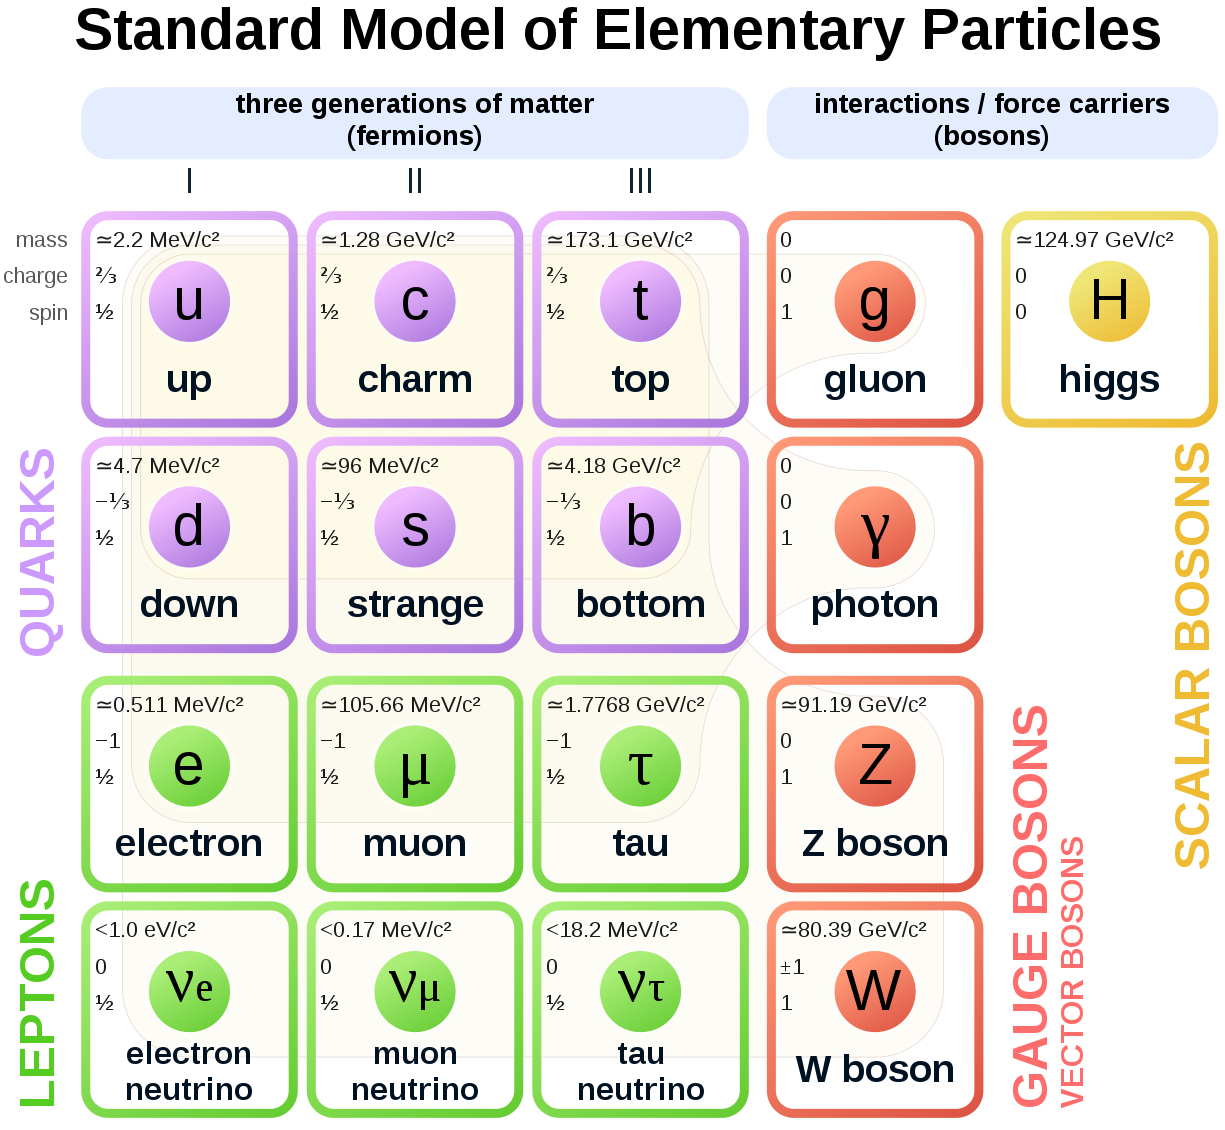
\includegraphics[width=0.5\textwidth]{Theory/SMv2}
%}
%\end{center}
\caption{Elementary particles of the SM.
%A display of the elementary particles described by the SM separated into their respective groups. 
Fermions are separated into quarks (purple) and leptons (green) and arranged into columns according to generation. The fourth and fifth columns show the Gauge (red) and Higgs (yellow) bosons, respectively. Approximate values of the masses are given.}
%The twelve fermions are separated into quarks (purple) and leptons (green) and arranged into three columns, per generation of matter particles. Gauge bosons (red) are shown as the fourth column, and the Higgs boson in the fifth. Approximate values of the masses are given. }
\label{fig:SMparticles}
%\end{figure}
\end{wrapfigure}
}

\newcommand{\HiggsMexicanHat}{
%\begin{wrapfigure}{R}{.5\textwidth}
\begin{figure}[!hbt]
\centering
%\begin{center}
%\subbottom[]{
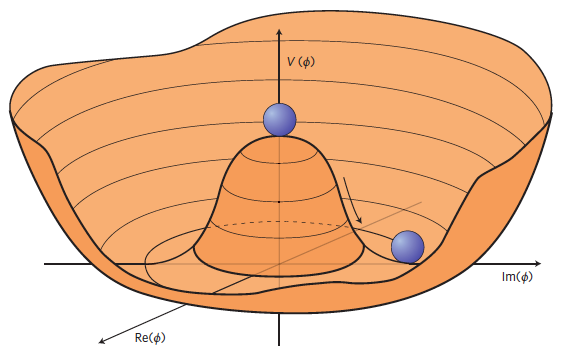
\includegraphics[width=0.5\textwidth]{Theory/HiggsMexicanHat}
%}
%\end{center}
\caption{Visualisation of the "Mexican hat" Higgs potential in the complex imaginary plane. The movement from teh centre of the potential to the trough corresponds to the massive Higgs boson~\cite{Ellis:2012465}.}
\label{fig:HiggsMexicanHat}
\end{figure}
%\end{wrapfigure}
}

\newcommand{\HiggsPlots}{
%\begin{wrapfigure}{R}{.5\textwidth}
\begin{figure}[!hbt]
%\centering
\begin{center}
\subbottom[]{
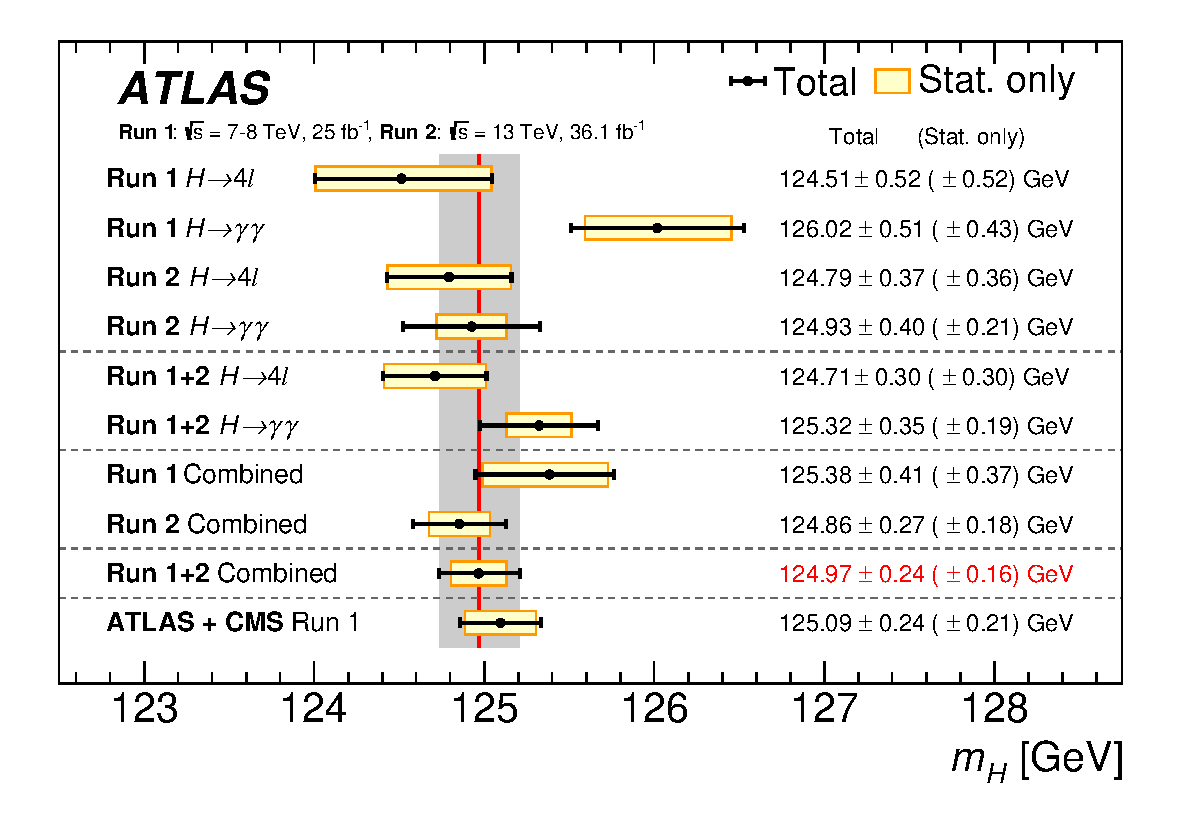
\includegraphics[width=0.49\textwidth]{Theory/Higgs_Run2_mass}
}
\subbottom[]{
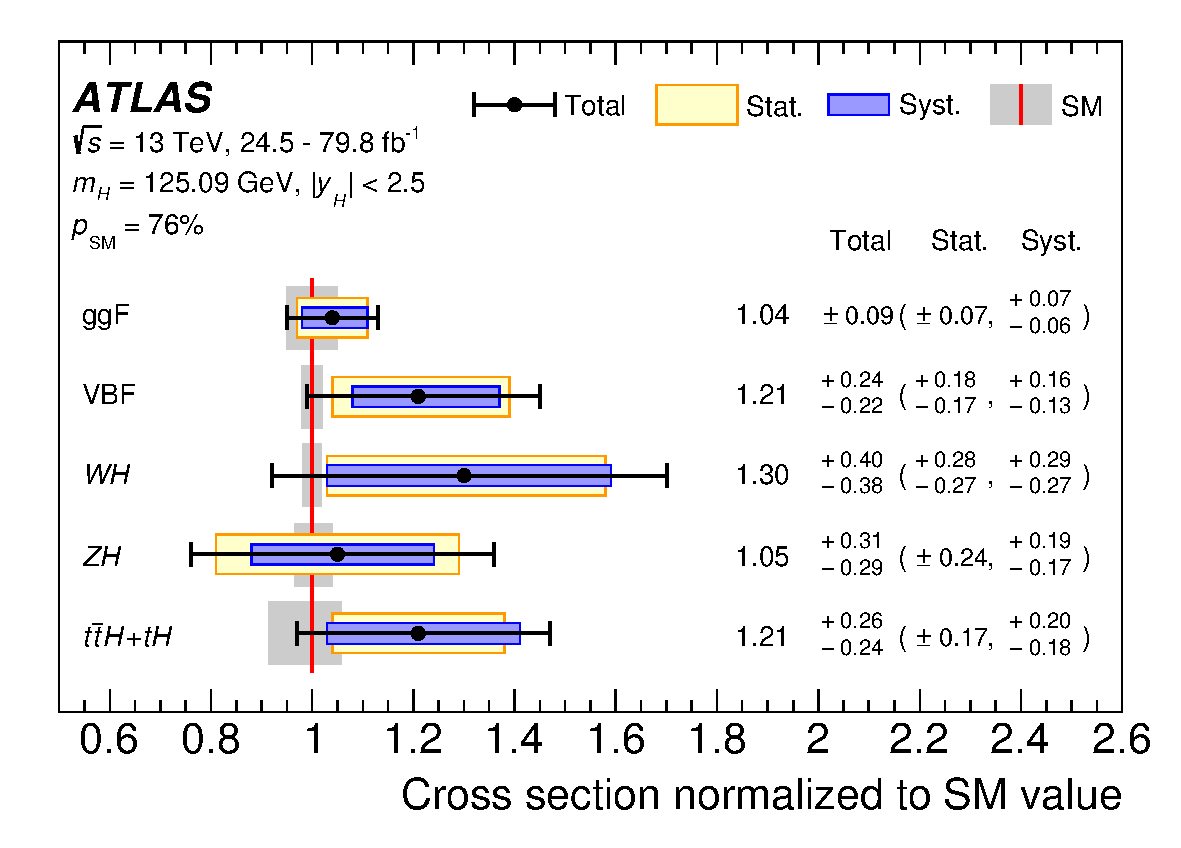
\includegraphics[width=0.469\textwidth]{Theory/Higgs_Run2_cross_sections}
}
\end{center}
\caption{(a) Summary of Higgs boson measurements from individual and combined analyses from \ac{ATLAS} and \ac{CMS} using Run 1 and Run 2 data. Statistical-only and total uncertainties are shown by horizontal yellow band and black error bars, respectively. Central value with corresponding total uncertainty for combined \ac{ATLAS} Run 1 +2 measurements are shown by the red vertical line and gray shaded column, respectively. Taken from Ref.~\cite{PhysRevD.101.012002}.
(b) Summary of Higgs boson cross-sections, normalised to their \ac{SM} predictions and with \ac{SM} branching fractions assumed. Total, systematic, and statistical uncertainties in measurements are shown by black error bars, blue boxes, and yellow boxes, respectively. The gray band indicate the theory uncertainty in the cross-section predictions. Taken from Ref.~\cite{2018345}. }
\label{fig:HiggsPlots}
\end{figure}
%\end{wrapfigure}
}

\newcommand{\HiggsLoopCorrection}{
%\begin{SCfigure}[1][!h]
%\centering
%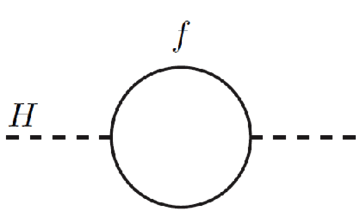
\includegraphics[width=0.4\textwidth]{Theory/1loopFermionicCorrections}
%\caption{One-loop fermionic quantum correction with coupling $\lambda_f$ to the Higgs mass.}
%\label{fig:HiggsLoopCorrection}
%\end{SCfigure}

\begin{figure}[!h]
\sidebysidecaption{0.55\textwidth}{0.4\textwidth}{%
  \caption{One-loop fermionic quantum correction with coupling $\lambda_f$ to the Higgs mass.}
   \label{fig:HiggsLoopCorrection}
}{%
  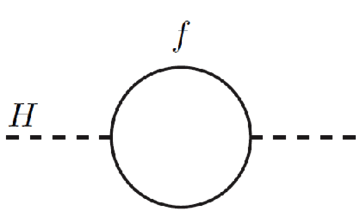
\includegraphics[width=\textwidth]{Theory/1loopFermionicCorrections}%
 
}
\end{figure}

}

\newcommand{\RunningConstant}{
%\begin{SCfigure}[1][!h]
%\centering
%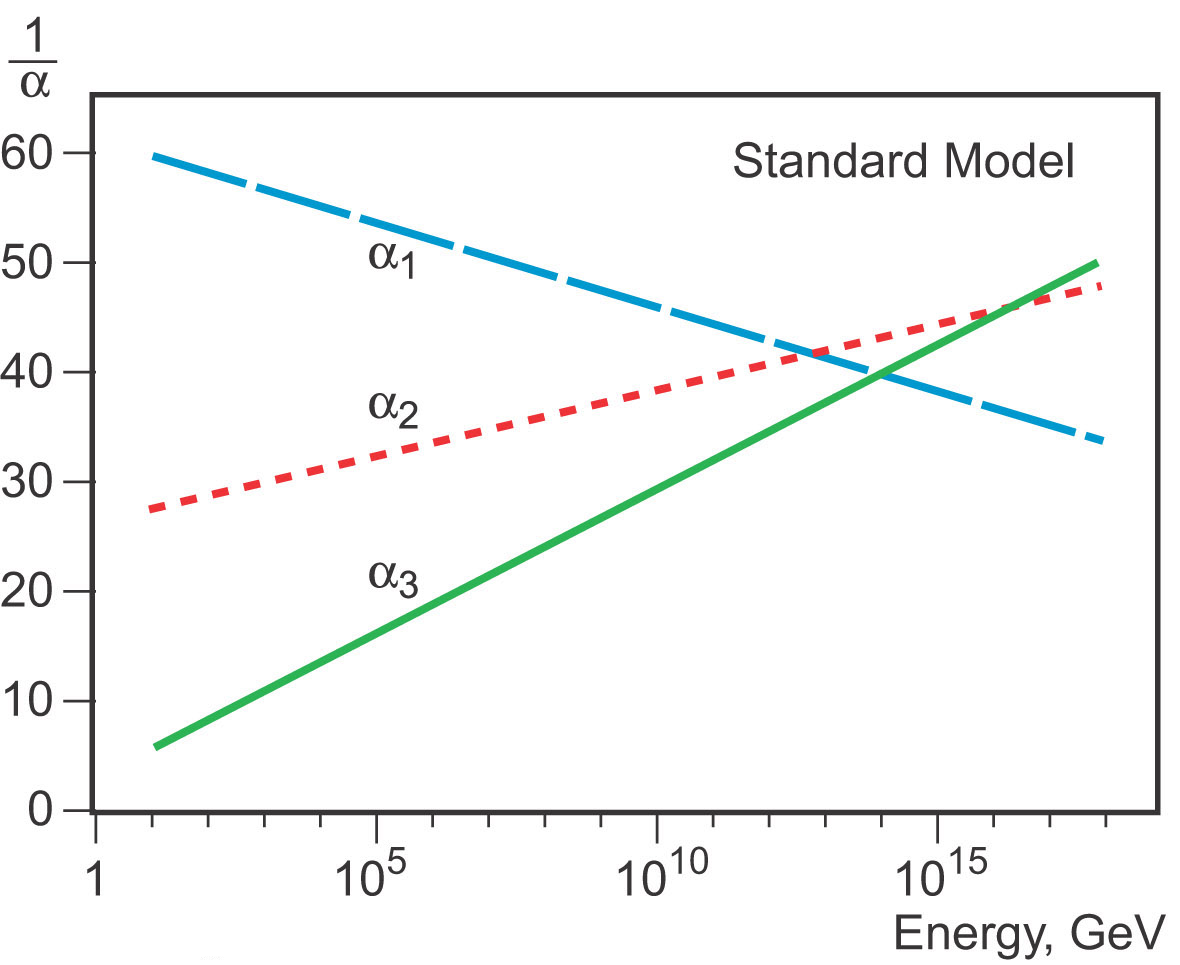
\includegraphics[width=0.4\textwidth]{Theory/RunningConstant}
%\caption{Running coupling constants of the electromagnetic (blue), weak (red) and strong(green) interactions in the \ac{SM}.}
%\label{fig:RunningConstant}
%\end{SCfigure}

\begin{figure}[!h]
\sidebysidecaption{0.5\textwidth}{0.42\textwidth}{%
    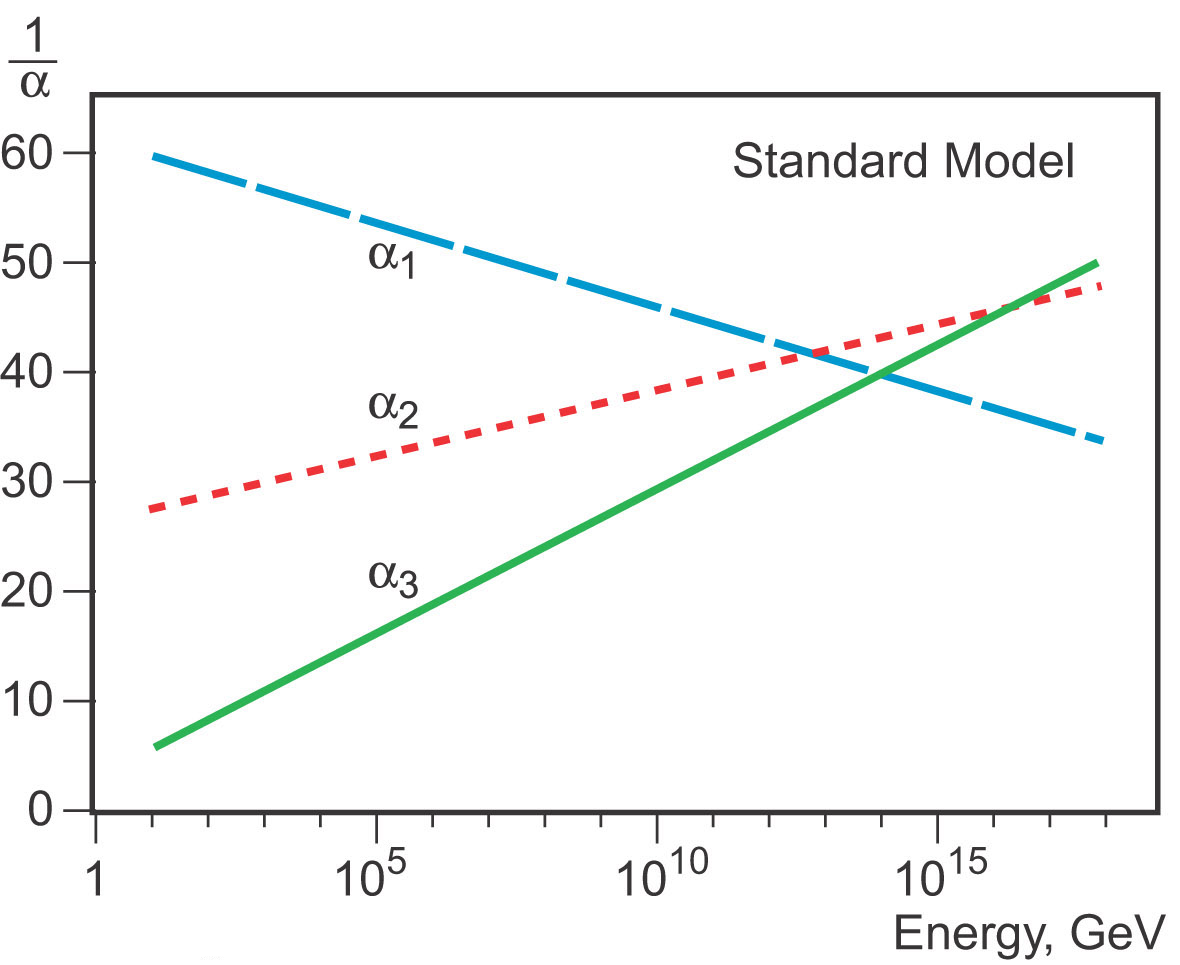
\includegraphics[width=\textwidth]{Theory/RunningConstant}%
}{%
  \caption{Running coupling constants of the electromagnetic (blue), weak (red) and strong(green) interactions in the \ac{SM}. The three lines do not converge, which goes against the idea of a \ac{GUT}.}
  \label{fig:RunningConstant}
}
\end{figure}

%begin{figure}[!h]
%\floatbox[{\capbeside\thisfloatsetup{capbesideposition={left,top},capbesidewidth=4cm}}]{figure}[\FBwidth]
%{\caption{Running coupling constants of the electromagnetic (blue), weak (red) and strong(green) interactions in the \ac{SM}.}\label{fig:RunningConstant}}
%{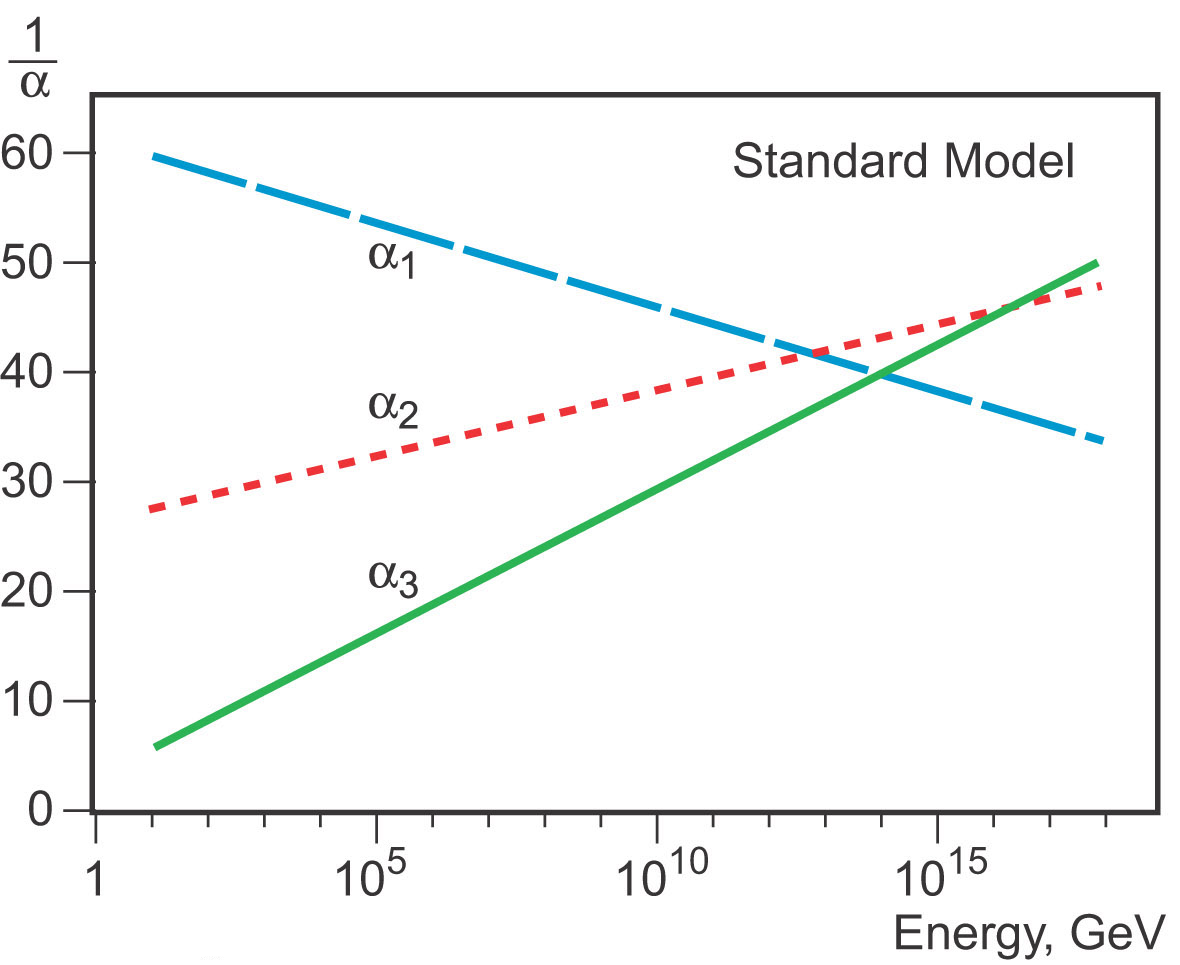
\includegraphics[width=0.4\textwidth]{Theory/RunningConstant}}
%\end{figure}

}

\newcommand{\GalaxyRotation}{
\begin{figure}[!h]
\sidebysidecaption{0.5\textwidth}{0.42\textwidth}{%
    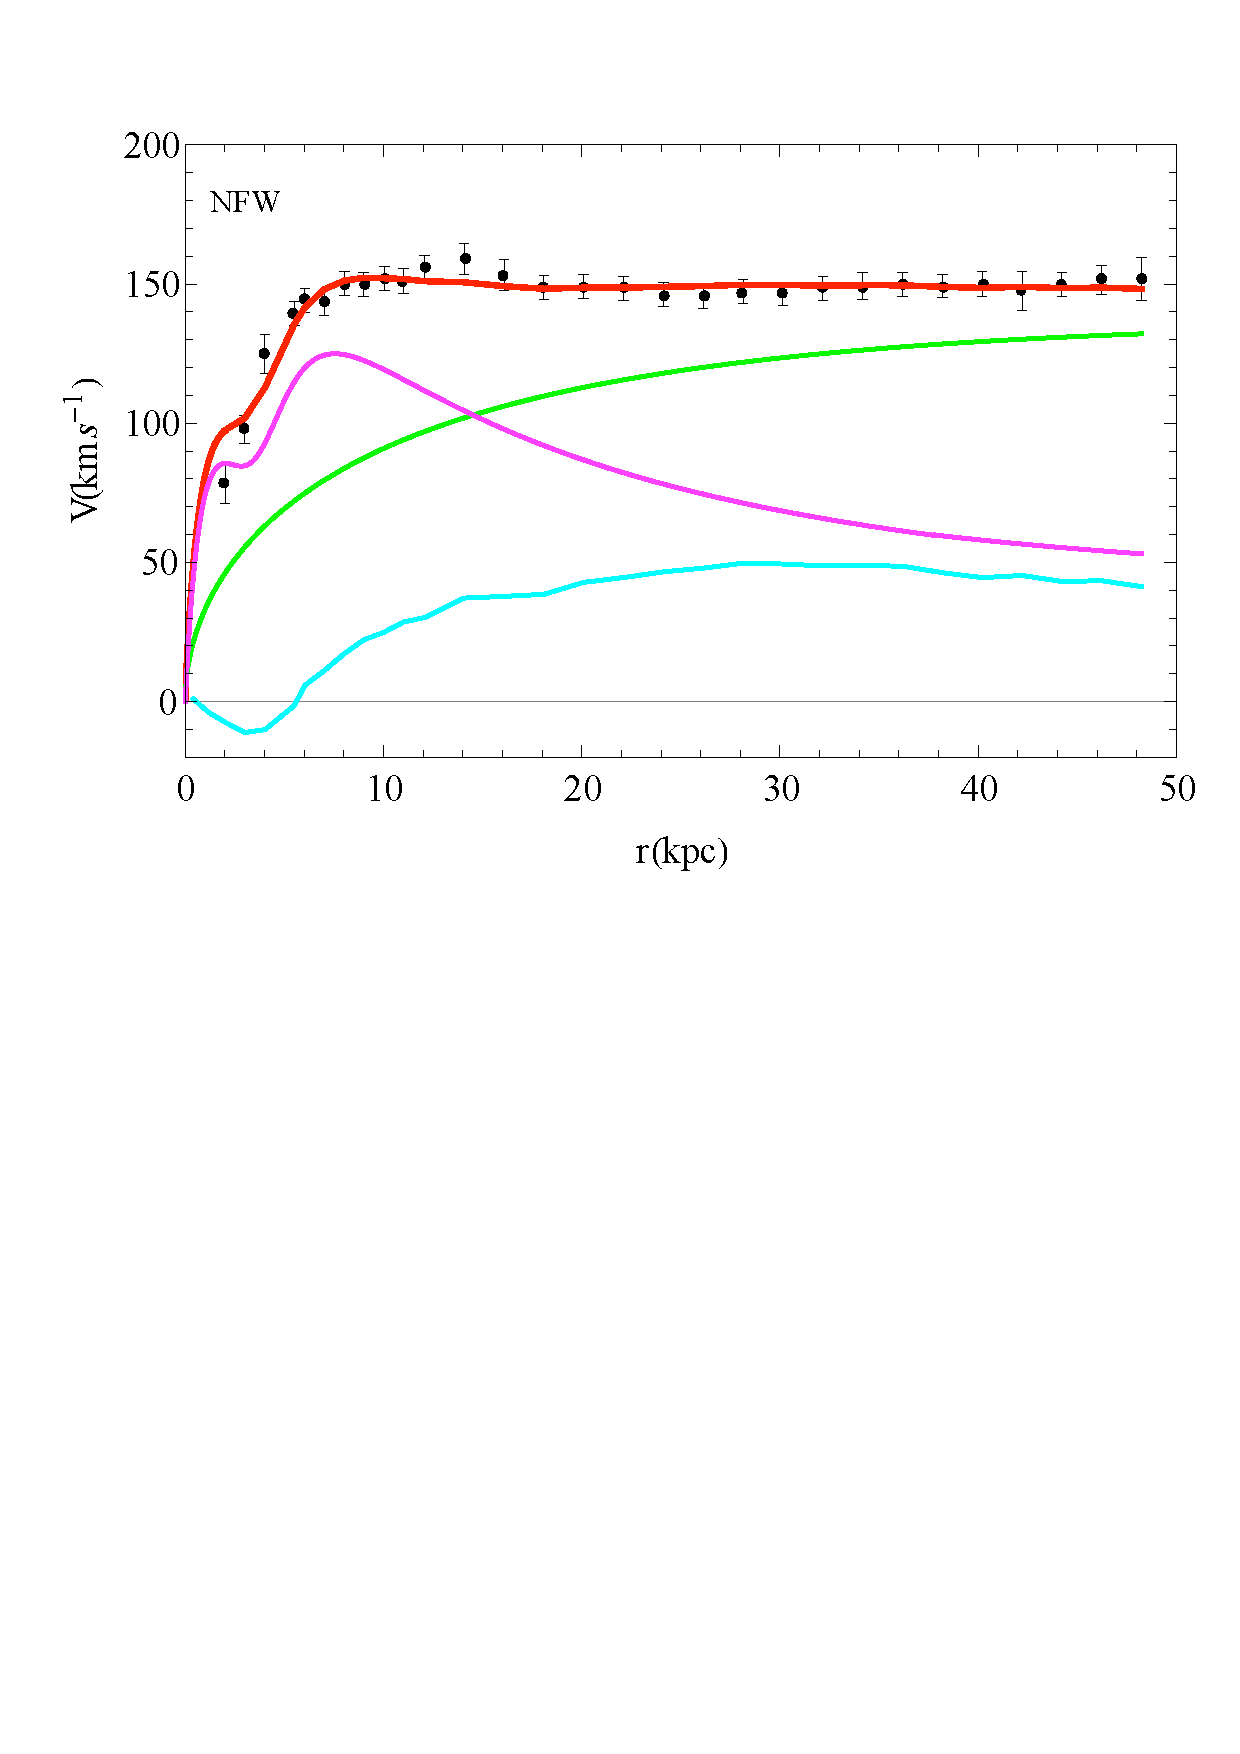
\includegraphics[width=\textwidth]{Theory/NFWGalaxyRotation}%
}{%
  \caption{Navarro, Frenken and White (NFW) \ac{DM} mass modelling for galaxy NGC 3198. Circular velocity data (black points with error bars) are shown with models for the stellar disk (magenta line), the \ac{DM} halo profile (green line), and the neutral Hydrogen contribution (azure line). The combination of contritions from all models is depicted by the thick red line, which shows that contribution from \ac{DM} is required  to account for the velocities observed at large radial distances.~\cite{galrot}}
  \label{fig:GalaxyRotation}
}
\end{figure}
}


\newcommand{\SUSYRunningConstant}{
%\begin{figure}[!h]
%\sidebysidecaption{0.5\textwidth}{0.42\textwidth}{%
%    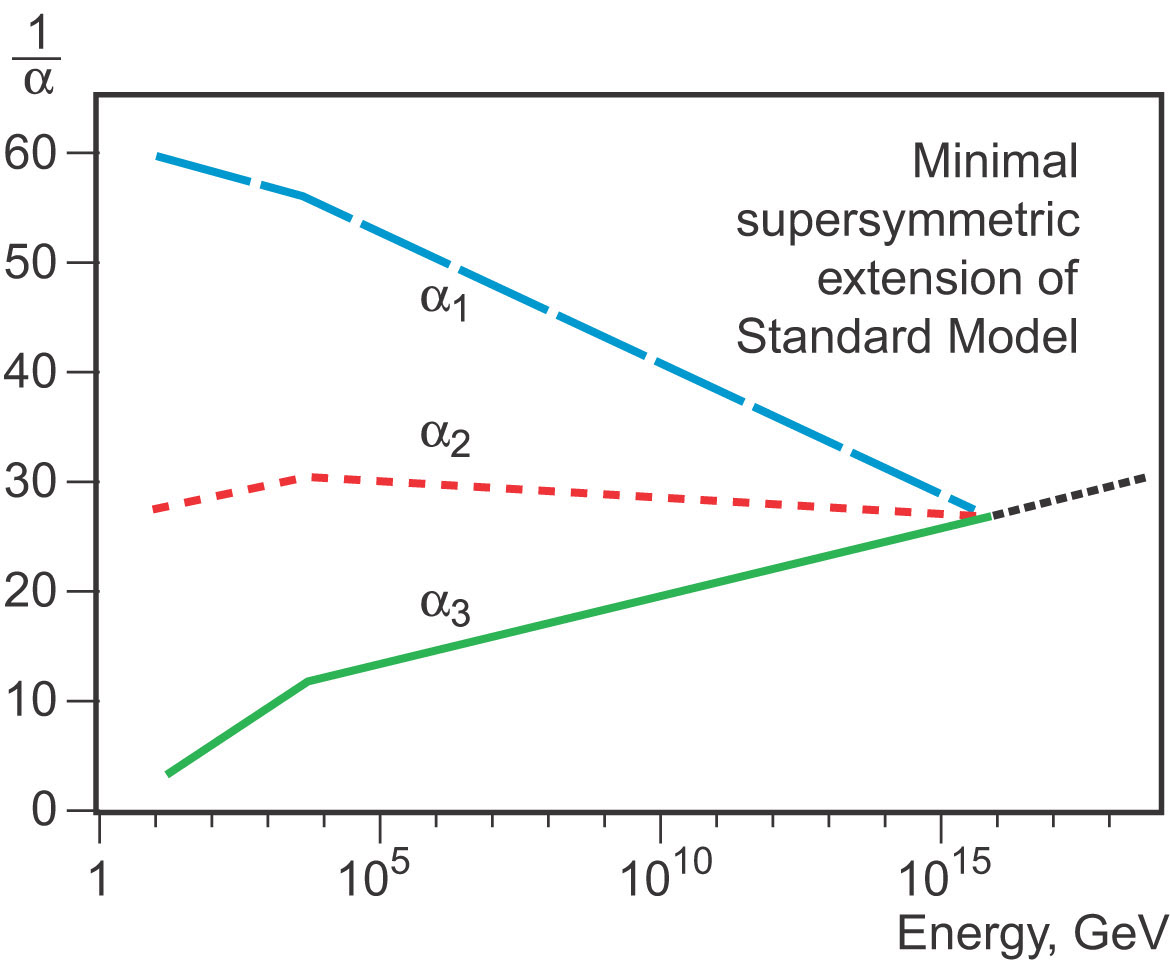
\includegraphics[width=\textwidth]{Theory/SUSYRunningConstant}%
%}{%
%  \caption{Running coupling constants of the electromagnetic (blue), weak (red) and strong(green) interactions in the \ac{MSSM}. The three lines converge in this model, this supporting a \ac{GUT}.}
%  \label{fig:SUSYRunningConstant}
%}
%\end{figure}

\begin{wrapfigure}{R}{.5\textwidth}
\centering
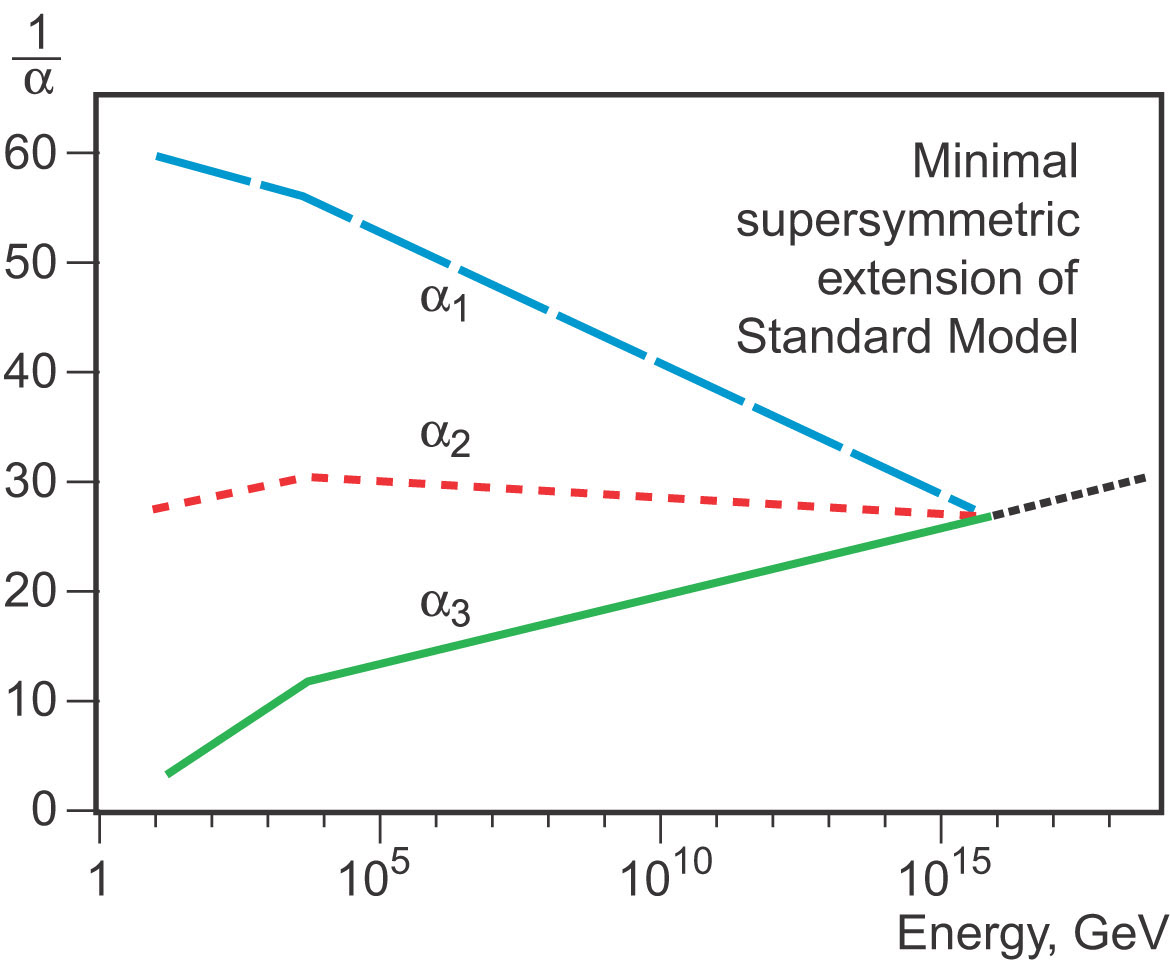
\includegraphics[width=0.5\textwidth]{Theory/SUSYRunningConstant}
\caption{Running coupling constants of the electromagnetic (blue), weak (red) and strong(green) interactions in the MSSM. The three lines converge in this model, this supporting a \ac{GUT}.}
\label{fig:SUSYRunningConstant}
\end{wrapfigure}

}

\newcommand{\SUSYewkfeynman}{
\begin{figure}[!h]
	\begin{center}
		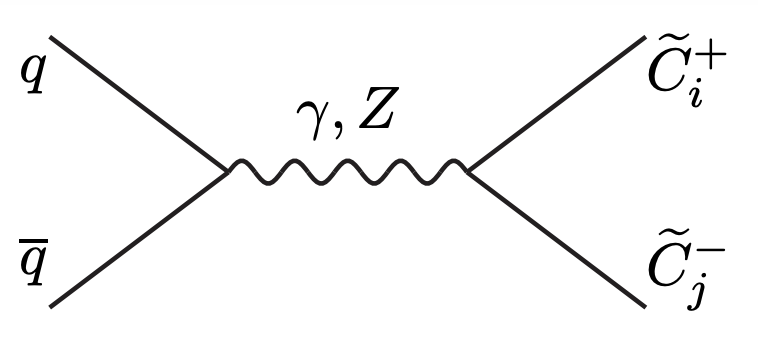
\includegraphics[width=0.3\textwidth]{Theory/analysis_SUSY_ewk_feynman_1}
		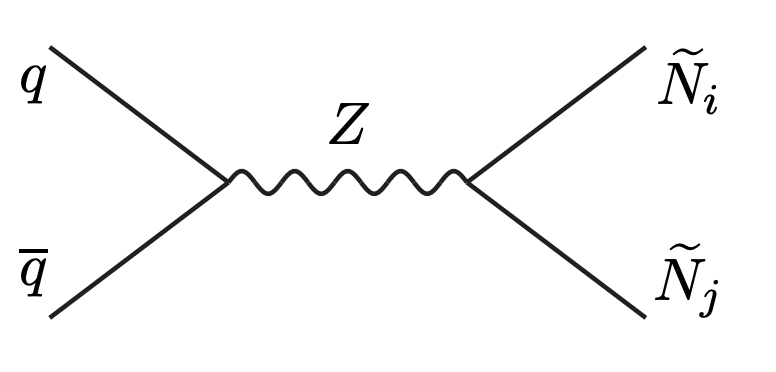
\includegraphics[width=0.3\textwidth]{Theory/analysis_SUSY_ewk_feynman_2}
		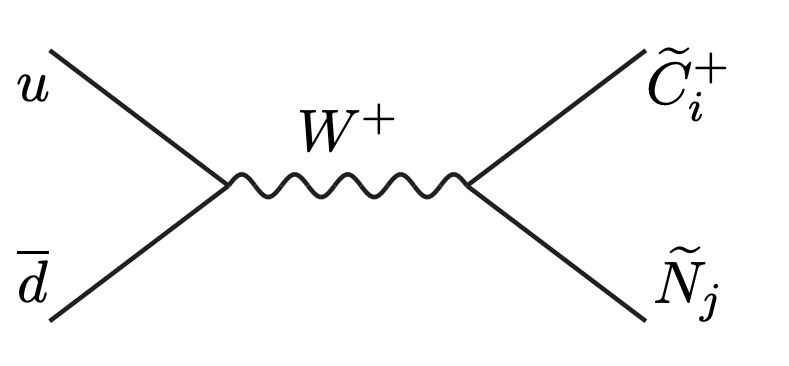
\includegraphics[width=0.3\textwidth]{Theory/analysis_SUSY_ewk_feynman_3}
		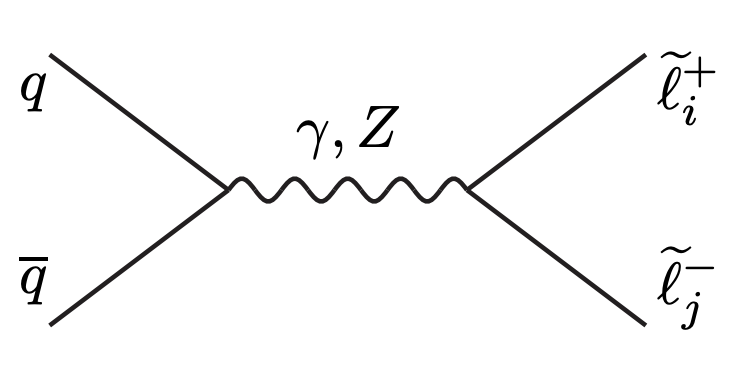
\includegraphics[width=0.3\textwidth]{Theory/analysis_SUSY_ewk_feynman_4}
		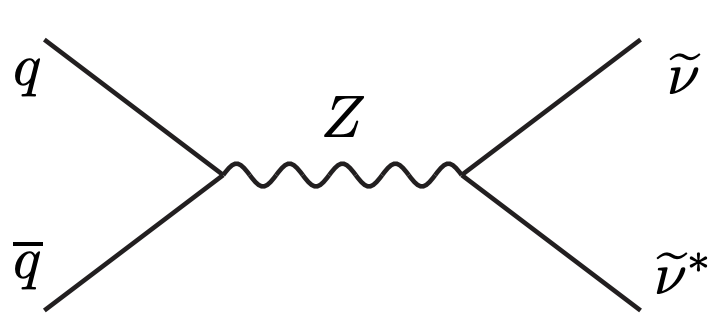
\includegraphics[width=0.3\textwidth]{Theory/analysis_SUSY_ewk_feynman_5}
		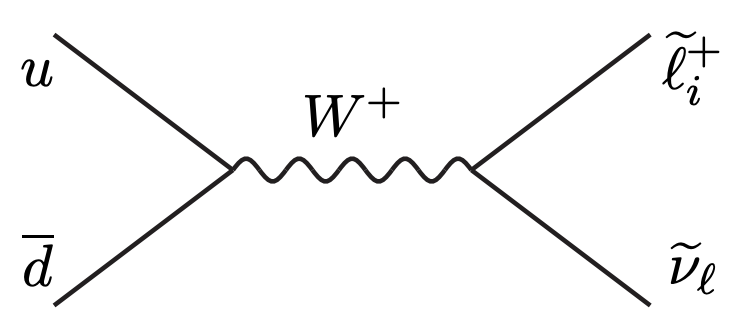
\includegraphics[width=0.3\textwidth]{Theory/analysis_SUSY_ewk_feynman_6}
	\end{center}
	\caption{Production channels of gauginos and sleptons with hadronic final states via electroweak mediators. For these diagrams $C^{\pm}_i=\chi_{i=1,2}^{\pm}$ and $N_j=\chi_{j=1,2,3,4}^{0}$~\cite{susyprimer}.}
\label{fig:SUSY_ewk_feynman}
\end{figure}
}

\newcommand{\SUSYcrosssection}{
\begin{figure}[!h]
	\centering
		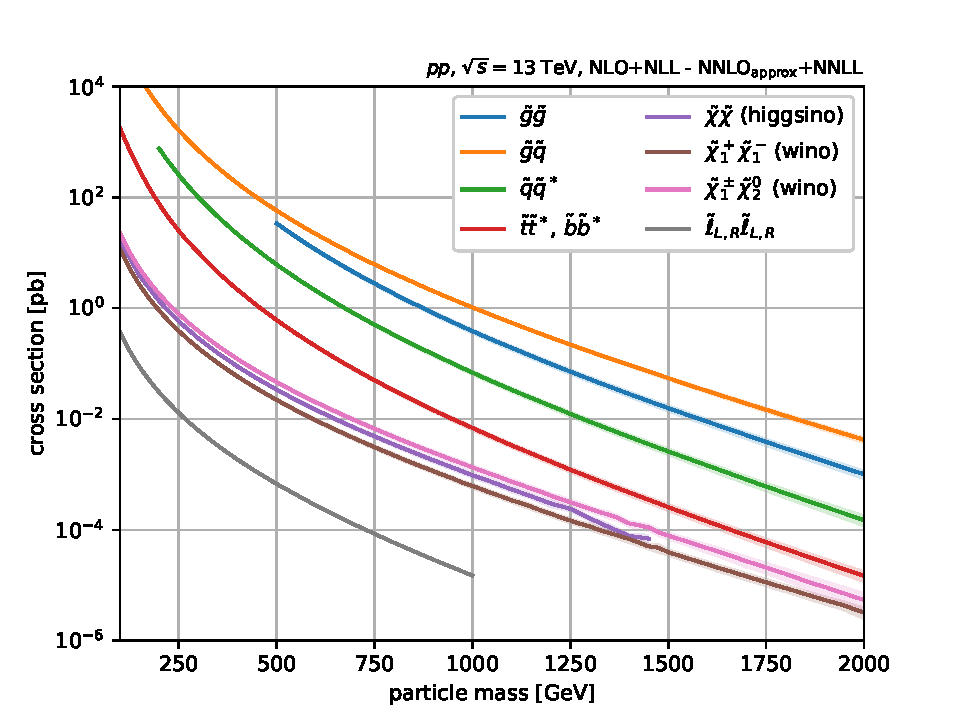
\includegraphics[width=0.8\textwidth]{Theory/theory_SUSY_cross_section}
	\caption{Theoretical cross-section values for sparticle production, as function of of their mass, in $pp$ collisions at \com$=13$ \tev. }
\label{fig:SUSY_cross_section}
\end{figure}
}

\newcommand{\StopExclusion}{
\begin{figure}[!h]
	\centering
		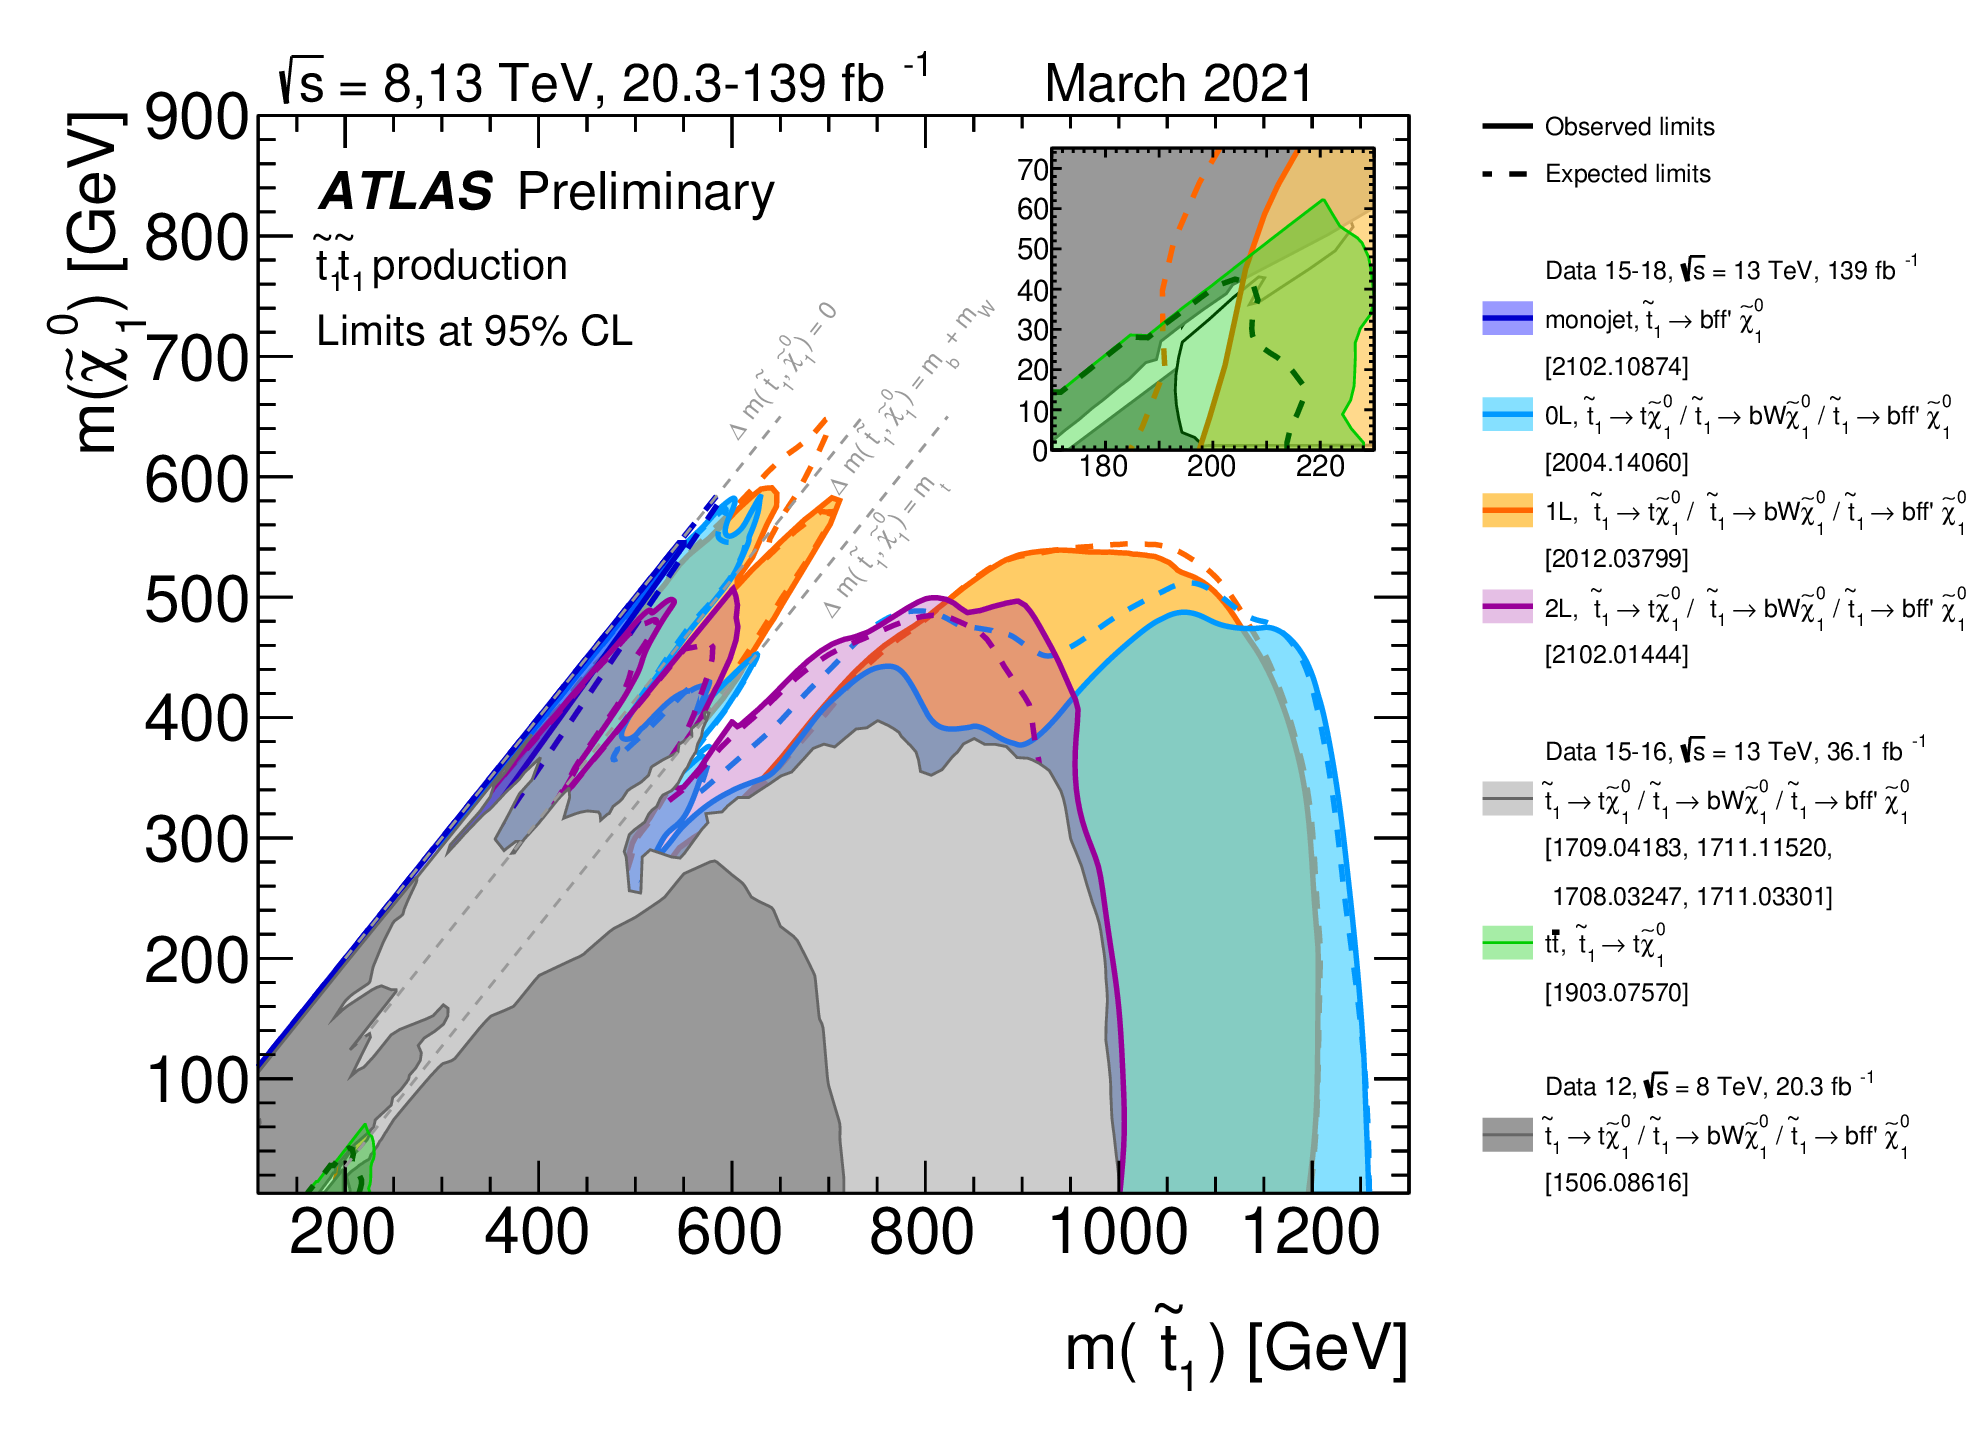
\includegraphics[width=\textwidth]{Theory/stop_exclusion}
	\caption{Observed and expected exclusion limits on the mass of the \stop\ squark. 
	Plots are produced using 20.3 \infb\ and 139 \infb\ of proton-proton collision data collected at \com$=8$ \tev\ and \com$=13$ \tev\ at the \ac{LHC}, by the \ac{ATLAS} experiment. Limits are set at the 95\% \ac{CL}.~\cite{ATL-PHYS-PUB-2021-007} }
\label{fig:stop_exclusion}
\end{figure}
}

\newcommand{\GluinoExclusion}{
\begin{figure}[!h]
	\centering
		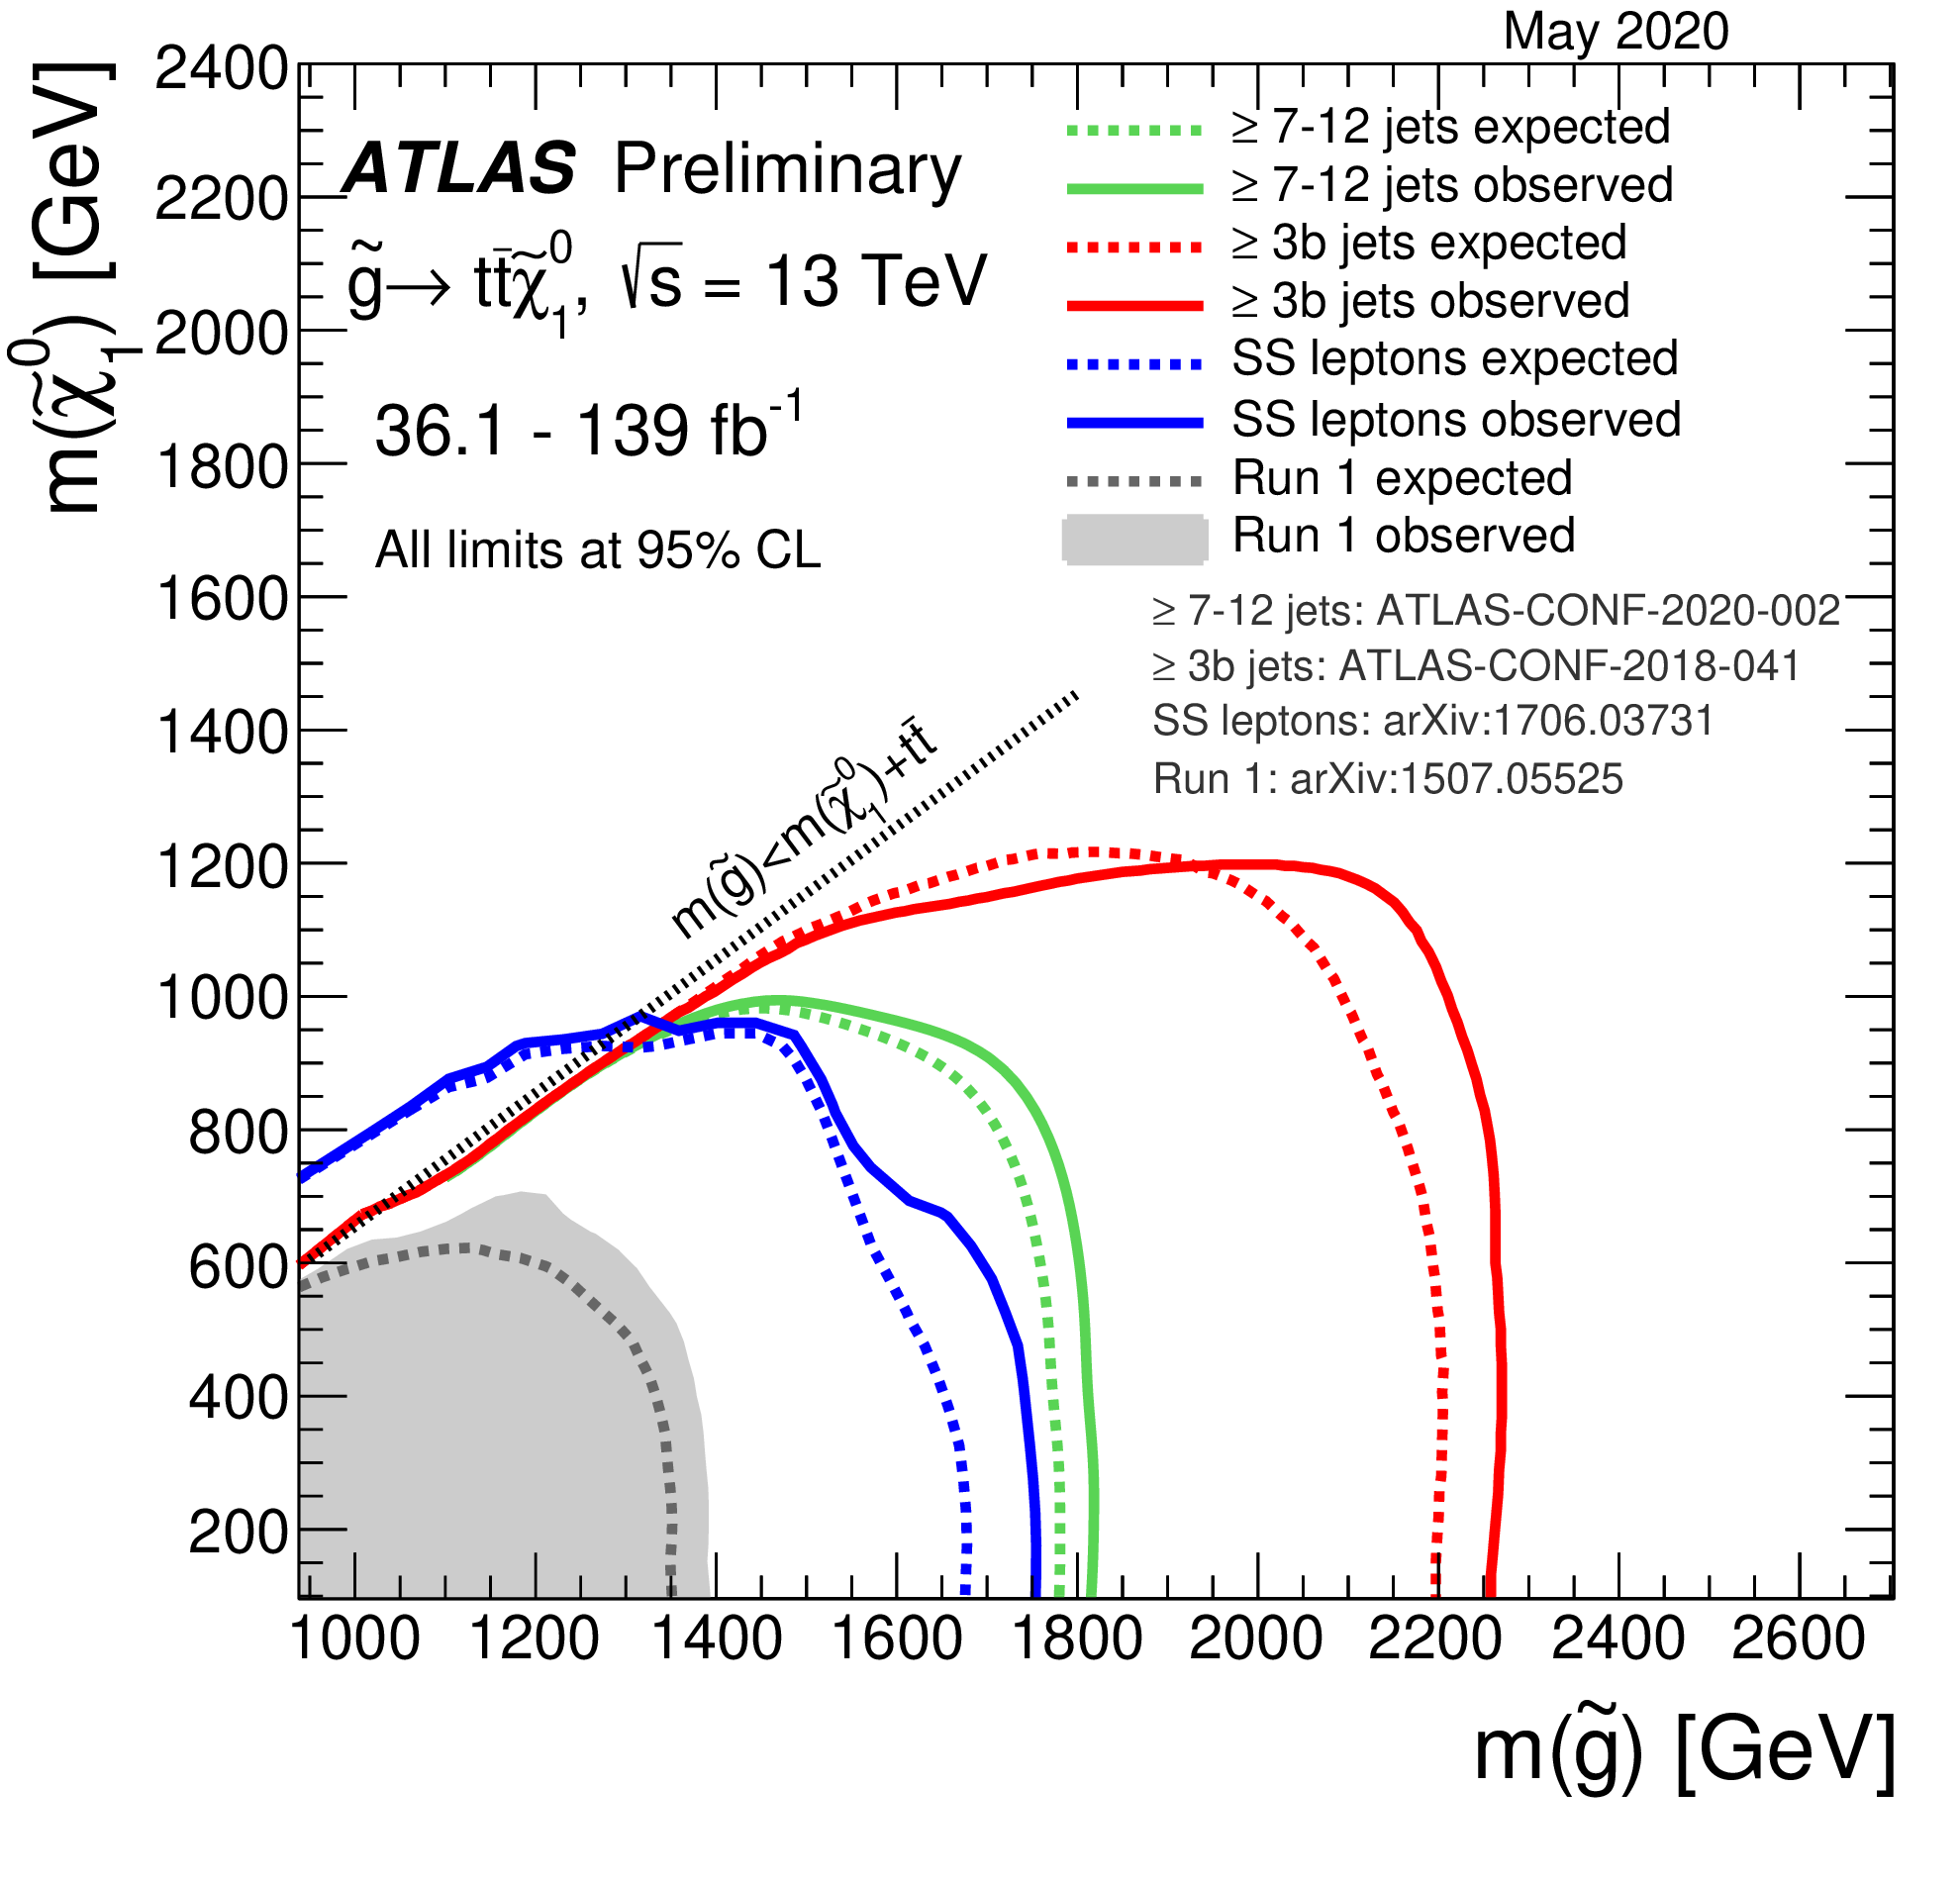
\includegraphics[width=0.7\textwidth]{Theory/gluino_exclusion}
	\caption{Observed and expected exclusion limits on the mass of the gluino (\gluino). 
	Plots are produced using 20.3 \infb\ and 139 \infb\ of proton-proton collision data collected at \com$=8$ \tev\ and $\sqrt{s}=13$ \tev\ at the \ac{LHC}, by the \ac{ATLAS} experiment. Limits are set at the 95\% \ac{CL}.~\cite{ATL-PHYS-PUB-2021-007} }
\label{fig:gluino_exclusion}
\end{figure}
}

%\newcommand{\FeynmanDiagramStau}{
%\begin{figure}[!hbt]
%\centering
%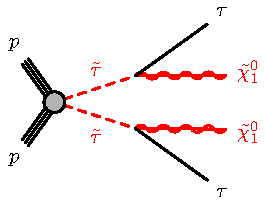
\includegraphics[width=0.7\textwidth]{Analysis/Feynman/staustau-tautauN1N1.pdf}
%\caption{Diagram of the decay topology of the signal model considered in this work. A pair production of charged staus and subsequent decay into two-tau final state.}
%\label{fig:feynman_direct_stau}
%\end{figure}
%}



	\section{The Standard Model} \label{sec:SM}
	
	 \SMparticles
	All the phenomena of particle physics, in terms of the properties and interaction of the known fundamental particles, is attempted to be explained by the \ac{SM}~\cite{MartinB.R.BrianRobert1997Pp}.
	The \ac{SM} describes all matter as composed by 4 distinct types of particles. 
	The first two are \textit{leptons} and \textit{quarks} and are spin-$\frac{1}{2}$ fermion, the third are a set of \textit{gauge bosons} that act as "force carriers", and the last is the Higgs boson. 
	There is good experimental evidence that supports the \ac{SM} of particle physics, as it was able to be used to successfully predict the existence of many particles including the W and Z bosons,
%	 the \ltau ,
	  and Higgs boson, all of which have been observed first at \ac{CERN}~\cite{WbosonDiscovery,ZbosonDiscovery,TauDiscovery,ATLASHiggs2012,CMSHiggs2012}.
	 
	
	 
	 The \ac{SM} is a \ac{QFT}~\cite{Peskin1995} that describes particles as excitations of their corresponding quantum field, which give rise to the particle's intrinsic physical properties (mass, charge, spin, colour etc...) and is able to describe the weak, electromagnetic and strong forces.%, although not gravity.
	 
	 The elementary particles described by the \ac{SM} can be generally classified by their spin properties.
	 \textit{Fermions}, which correspond to leptons and quarks and are generally referred to as "matter" particles, possess half-integer spin in units of $\hbar$, while \textit{bosons}, known as the "information" carrier, have integer-spin values. 
	 The spin-1 bosons are known as the gauge bosons and are generally considered as the "force" mediators.
	 Figure~\ref{fig:SMparticles} shows the elementary particles of the \ac{SM} known today, separated into the different groups described above.
	 
	 \subsection*{Symmetries and Gauge Groups}
	As mentioned in the previous section, the \ac{SM} uses \ac{QFT} to describe particle dynamics by Lagrangian field densities:% $\pazocal{L}$:
	\begin{equation}
	\pazocal{L}=\pazocal{L}(\varphi,\partial_{\mu}\varphi),
	\end{equation}
	where $\varphi$ is a fermion field and $\partial_{\mu}\varphi$ is the partial derivative four-vector of all generalised spatial coordinates. The equations of motion of a system, as described using Lagrangian formalism, are derived by minimising the action $\pazocal{S}$, where:
	\begin{equation}
\pazocal{S} = \int \pazocal{L}dt.
	\end{equation}
	Noether's theorem states that every differentiable symmetry of the action of a physical system, $\pazocal{S}$, has a corresponding conservation law~\cite{doi:10.1080/00411457108231446}. 
	Here, a symmetry is a property of a physical system that under certain transformations remains preserved.

	The \ac{SM} is described as a \ac{QFT} \textit{gauge theory}, meaning that its Lagrangian is invariant under a set of gauge transformations~\cite{lederman2004symmetry}. 
	A gauge transformation is a continuous set of local transformations between all possible gauges, forming a \textit{Lie group}, which can be represented through a basis of linear transformations. 
	For each group generator associated to any Lie group, a corresponding \textit{gauge field} emerges.
	These fields relate to the symmetry transformations at different points in space-time, and their corresponding quanta are called \textit{gauge bosons}.

	The full \ac{SM} gauge symmetry group can be described as:
		\begin{equation}
		U(1)_{Y} \otimes SU(2)_L \otimes SU(3)_C,
		\label{eq:SM}
		\end{equation}
	where each term represents a symmetry group to which the strong, \ac{EM} and weak interactions can be associated.
	In equation~\ref{eq:SM}, $Y$ represents the hypercharge, which relates the electric charge ($Q$) to the third component of the weak isospin ($I_3$) via the Gell-Mann-Nishijima formula $Q=I_3+\frac{1}{2}Y$~\cite{GMformula,Nformula}. The "handedness" is represented by $L$, while the colour charge by $C$. 
	Handedness refers to the relative direction of helicity with respect to the direction of momentum, so that a system whose spin direction is the same as the momentum is called "right-handed", and one with opposite directions is called "left-handed".
	$I_3$ can either be $+\frac{1}{2}$ or 0 for right-handed or for left-handed particles, respectively.
	\subsection*{Fermions}
	The \ac{SM} attempts to describe all physical matter\footnote{with some note-worthy exceptions such as dark matter which will be discussed later in the chapter} using twelve particles, called fermions, separated into two groups, quarks and leptons. Within each group, the particles can be further separated into three sets of $SU(2)_L$ weak isospin doubles, called \textit{generations}, that change with increasing mass. 
	%Each quark generation contains one up- and one down-type quark, while lepton generations contain one charge and one neutral lepton.
	%The \ac{SM} fermions can be organised into the three generation of $SU(2)_L$ weak isospin doubles, with quarks denoted as:
	Quarks can be denoted as:
	%\begin{equation}
		\begin{equation}
			\begin{pmatrix} u \\ d \end{pmatrix}_L\quad 
			\begin{pmatrix} c \\ s \end{pmatrix}_L\quad 
			\begin{pmatrix} t \\ b \end{pmatrix}_L, 
			\label{eq:quarks}
		\end{equation}
	where each flavour pair consists of an "up" (\textit{up}, \textit{charm}, \textit{top}) and "down" (\textit{down}, \textit{strange}, \textit{bottom}) type, with a charge of $+\frac{2}{3}$ and $-\frac{1}{3}$ in units of electron charge ($e$), respectively. 
	The corresponding anti-quark particles have opposite charges of $-\frac{2}{3}$ for the \textit{anti-up} ($\bar{u}$), \textit{anti-charm} ($\bar{c}$) and \textit{anti-top} ($\bar{t}$), and $+\frac{1}{3}$ for \textit{anti-down} ($\bar{d}$), \textit{anti-strange} ($\bar{s}$), and \textit{anti-bottom} ($\bar{b}$), in units of $e$.
	Analogously to electric charge, quarks also have colour charge, which exists in three different states, \textit{red} \textit{green} and \textit{blue}. Quarks cannot propagate as free particles but must instead be grouped into colourless hadronic matter, known as \textit{hadrons}. Hadrons composed of quark-antiquark pairs (\eg\  the \textit{pions} $\pi^0$, $\pi^{\pm}$) are know \textit{mesons} while three-quark hadrons (\eg\ protons and neutrons) are known as \textit{baryons}. In Addition to the electric charge, $Q$, quarks have another characteristic quantum number called Baryon number, ($B$), with a value of $\frac{1}{3}$ ($-\frac{1}{3}$) for each quark (anti-quark) that must be conserved in all known interactions.
		 
		Similarly to quarks, leptons can also be grouped by generation into:
		\begin{equation}
			\begin{pmatrix} \nu_e      \\ e^-    \end{pmatrix}_L \quad
			\begin{pmatrix} \nu_{\mu}  \\ \mu^-  \end{pmatrix}_L \quad
			\begin{pmatrix} \nu_{\tau} \\ \tau^-  \end{pmatrix}_L,
			\label{eq:leps}
		\end{equation}
		%Each doublet corresponds to a familiar flavour pair, with quarks paired into "up" (\textit{up}, \textit{charm}, \textit{top}) and "down" (\textit{down}, \textit{strange}, \textit{bottom/beauty}) types, with a charge of $+\frac{2}{3}$ and $-\frac{1}{3}$ of the electron charge, respectively.
		where a chargeless neutrino ($\nu$) is assigned for each charged lepton: \textit{electron} ($e$), \textit{muon} ($\mu$), and \textit{tau} ($\tau$). Each lepton has a characteristic quantum number, similar to the Baryon number, which must be conserved in all interactions, called Lepton number. There are three types of lepton numbers, according to each lepton type ($L_e$, $L_{\mu}$, $L_{\tau}$) with values of 1 or -1 for leptons or anti-leptons, respectively.
		
		For the quarks and leptons shown in ~\ref{eq:quarks} and ~\ref{eq:leps}, $L$ denotes the "left-handedness" of the fermions, for which there are also corresponding "right-handed" singlets, with the exception of neutrinos (anti-neutrinos) which are uniquely left-handed (right-handed).
		
		A summary of the quarks and leptons described above along with their relative characteristic quantum numbers is given in table~\ref{tab:quarks_n_leps}.
	\begin{table}[!hbt]
	\centering
	\caption{Summary of quarks and leptons described in the \ac{SM} with corresponding symbols, charge, and Baryon/Lepton quantum numbers given. Anti-particles posses same quantum properties but with opposite sign.}
	\resizebox{\textwidth}{!}{
	%\documentclass[10pt]{article}
%\usepackage[usenames]{color} %used for font color
%\usepackage{amssymb} %maths
%\usepackage{amsmath} %maths
%\usepackage[utf8]{inputenc} %useful to type directly diacritic characters
%\usepackage{multirow}\begin{document}
%% Please add the following required packages to your document preamble:
%% \usepackage{multirow}
%\begin{table}[]
\begin{tabular}{lcccccc}
\hline
\multirow{2}{*}{Quarks} & \multirow{2}{*}{Symbol} & \multirow{2}{*}{\begin{tabular}[c]{@{}c@{}}Charge\\ ($Q$)\end{tabular}} & \multirow{2}{*}{\begin{tabular}[c]{@{}c@{}}Baryon \\ Number \\ ($B$)\end{tabular}} & \multicolumn{3}{c}{\begin{tabular}[c]{@{}c@{}}Lepton \\ Number\end{tabular}} \\
 &  &  &  & \begin{tabular}[c]{@{}c@{}}($L_e$,\\ \quad\end{tabular} & \begin{tabular}[c]{@{}c@{}}$L_{\mu}$,\\ \quad\end{tabular} & \begin{tabular}[c]{@{}c@{}}$L_{\tau}$)\\ \quad\end{tabular} \\ \hline \hline
up & u & $+\frac{2}{3}$ & $\frac{1}{3}$ & 0 & 0 & 0 \\
charm & c & $+\frac{2}{3}$ & $\frac{1}{3}$ & 0 & 0 & 0 \\
top & t & $+\frac{2}{3}$ & $\frac{1}{3}$ & 0 & 0 & 0 \\
down & d & $-\frac{1}{3}$ & $\frac{1}{3}$ & 0 & 0 & 0 \\
strange & s & $-\frac{1}{3}$ & $\frac{1}{3}$ & 0 & 0 & 0 \\
bottom & b & $-\frac{1}{3}$ & $\frac{1}{3}$ & 0 & 0 & 0 \\ \hline
\end{tabular}
%\end{table}
%\end{document}	
	\quad
	%\documentclass[10pt]{article}
%\usepackage[usenames]{color} %used for font color
%\usepackage{amssymb} %maths
%\usepackage{amsmath} %maths
%\usepackage[utf8]{inputenc} %useful to type directly diacritic characters
%\usepackage{multirow}\begin{document}
%% Please add the following required packages to your document preamble:
%% \usepackage{multirow}
%\begin{table}[]
\begin{tabular}{lcccccc}
\hline
\multirow{2}{*}{Lepton} & \multirow{2}{*}{Symbol} & \multirow{2}{*}{\begin{tabular}[c]{@{}c@{}}Charge\\ ($Q$)\end{tabular}} & \multirow{2}{*}{\begin{tabular}[c]{@{}c@{}}Baryon \\ Number \\ ($B$)\end{tabular}} & \multicolumn{3}{c}{\begin{tabular}[c]{@{}c@{}}Lepton \\ Number\end{tabular}} \\
 &  &  &  & \begin{tabular}[c]{@{}c@{}}($L_e$,\\ \quad\end{tabular} & \begin{tabular}[c]{@{}c@{}}$L_{\mu}$,\\ \quad\end{tabular} & \begin{tabular}[c]{@{}c@{}}$L_{\tau}$)\\ \quad\end{tabular} \\ \hline \hline
electron & $e$ & -1 & 0 & 1 & 0 & 0 \\
muon & $\mu$ & -1 & 0 & 0 & 1 & 0 \\
tau & $\tau$ & -1 & 0 & 0 & 0 & 1 \\
electron neutrino & $\nu_{e}$ & 0 & 0 & 1 & 0 & 0 \\
muon neutrino & $\nu_{\mu}$ & 0 & 0 & 0 & 1 & 0 \\
tau neutrino & $\nu_{\tau}$ & 0 & 0 & 0 & 0 & 1 \\ \hline
\end{tabular}
%\end{table}
%\end{document}	
	}
	\label{tab:quarks_n_leps}
	\end{table}
	
%	\end{equation}
	
	%			&\left( u \atop d \right)\, , \left( c \atop s \right)\, , \left( t \atop b \right) \\
%			&\left( e \atop \nu_e \right)\, , \left( \mu \atop \nu_{\mu} \right)\, , \left( \tau \atop \nu_{\tau} \right) 	
	
	\subsection*{Electromagnetic Interactions}
	The electromagnetic interactions are described in the \ac{SM} by \ac{QED}, and are mediated by the photon ($\gamma$).
	\ac{QED} is an \textit{abelian} gauge theory described by the symmetry group $U(1)$, meaning that the $1\times1$ generator is able to only self-commute, resulting in the fact that the electrically neutral photon is unable to self-interact~\cite{Pich2012}. The electromagnetic force affects fermions (with the exception of neutrinos, which are only affected by the weak force) via the exchange of photons, with a coupling constant value of 
	\begin{equation}
	\alpha_{EM}=\frac{e^2}{4\pi}\sim\frac{1}{137},
	\end{equation}
	 where $e$ is the electric elementary charge.	
	\subsection*{Weak Interactions}
	The weak force interactions, described by Equation~\ref{eq:SM} by the $SU(2)_L$ term, is associated to the "handedness" of the particles and behaves in a non-abelian nature. This means that the three $2\times2$ generators of which the $SU(2)_L$ group is comprised of, do not commute.
	The weak interaction, thus, only couples with left-handed chiral fields via the $W$ boson, which correspond to the charged current, while both left- and right-handed chiral fields can couple to the $Z$ boson, that corresponds to the neutral current. 
	Even though both leptons and quarks have both left- and right-hand components, neutrinos (anti-neutrinos) only have the left-handed (right-handed) component observable in nature. 
	The consequence of this is that the $W$ boson coupling is the only interaction that can change quark flavour, and can also violate both \textit{parity} and \textit{charge-parity} symmetry~\cite{Weinberg:1996kr}.  
	
	The weak force mediators have also significant masses, as show in table~\ref{tab:bosons}, which results in short life-spans of $\pazocal{O}(10^{-25}\mathrm{s})$. Consequently the weak force acts on relatively short distances of $\pazocal{O}(10^{-18}\mathrm{m})$. The coupling constant of the weak interaction at zero momentum transfer is:
	\begin{equation}
	\alpha_{weak}\sim\frac{1}{30}
	\end{equation}
	\subsection*{Strong Interactions}
	The theory that describes the strong interactions in the \ac{SM}, \ie\ the $SU(3)_C$ symmetry group in Equation~\ref{eq:SM}, is the \ac{QCD}.
	In \ac{QCD}, the strong force is mediated by the massless and electrically neutral \textit{gluon} ($g$), which couples to the quark's quantum property known as colour charge.
	Colour charge allows quarks to be described as color triplets (\textit{red},\textit{green}, \textit{blue}), each with identical strong interactions, which allow colours of the same quark flavour to exist in the same bound state without violating the Pauli exclusion principle.
	This leads to three important features of \ac{QCD}:
	\begin{itemize}
	\item[]\textit{Confinement:} all quarks are bound to colourless hadrons and cannot be observed as free particles.  This can be achieved with the combination of three quarks (anti-quarks) with all three colours (anti-colours) in \textit{baryons}, or as \textit{mesons} where the colour and baryon number cancel.
	 \item[]\textit{Hadronisation:} gluons are non-abelian, meaning that they can self-interact and generate virtual gluons in quantities proportional to the distance between the two interacting quarks. This gives the strong force a range of $\pazocal{O}(10^{-15}\mathrm{m})$, but with an increasing force strength as the distance also increases.
	As the energy required to separate the two quarks increases, there comes a point at which it is energetically preferable to produce a pairs of hadrons from the vacuum, than to increases the distance any further. The continuous production of hadrons, which form a "jet" cone, proceeds until the energy is low enough to form bound hadron states.
	\item[]\textit{Asymptotic freedom:} the strong force coupling constant ($\alpha_S$) is the strongest of all the forces described, where $\alpha_S=1$ at zero momentum transfer.
	 However, $\alpha_S$ is also correlated to the four-momentum squared ($Q^2$), where
%	\footnote{The four-momentum is a 4-dimensional vector used to describe the energy and momentum of particle in the 3-dimensional space such that $\vec{Q}=\begin{pmatrix}E \\ p_x c \\ p_y c \\ p_z c \end{pmatrix}$ } 
	the four-momentum vector ($\vec{Q}$) describes the energy and momentum of a particle in 3-dimensional space, and the length of the four-momentum vector is associated to the rest energy of the particle. The correlation between $\alpha_S$ and $Q^2$ can be given to a good approximation by:
	\begin{equation}
	\alpha_S\propto \frac{1}{n_f \mathrm{log}\left(\frac{Q^2}{\Lambda_{QCD}^2}\right)},
	\end{equation}
	where $n_f$ is the number of quarks with mass below $Q^2$ and $\Lambda_{QCD}$ is the \ac{QCD} characteristic scale, for $Q^2>>\Lambda_{QCD}^2$. As $Q^2$ approaches $\Lambda_{QCD}$, the value of $\alpha_S$ will quickly diverge.
	 As such, \ac{QCD} cannot be described at low energies using perturbation theory. 
	 On the other hand, at high energy scales $\alpha_S$ becomes sufficiently small, such that perturbation theory can be applied and the interactions between quarks and gluons becomes weaker, enabling quarks to behave as free particles.
	\end{itemize}		 
	
	The properties and mediators described in the above sections are summarised in Table~\ref{tab:bosons}.
	\begin{table}[!hbt]
	\centering
	\caption{Summary of the forces and mediations  described in the \ac{SM} with corresponding masses and charge values.}
	%\resizebox{\textwidth}{!}{
	%\documentclass[10pt]{article}
%\usepackage[usenames]{color} %used for font color
%\usepackage{amssymb} %maths
%\usepackage{amsmath} %maths
%\usepackage[utf8]{inputenc} %useful to type directly diacritic characters
%\usepackage{multirow}
%\begin{document}
%% Please add the following required packages to your document preamble:
%% \usepackage{multirow}
%\begin{table}[]
\begin{tabular}{ccccc}
\hline
Force & Name & Symbol & \begin{tabular}[c]{@{}c@{}}Mass\\ $[\mathrm{GeV}]$\end{tabular} & \begin{tabular}[c]{@{}c@{}}Charge\\ $[e]$\end{tabular} \\ \hline \hline 
Electromagnetic & Photon & $\gamma$ & 0 & 0 \\ \hline
\multirow{2}{*}{Weak} & W & $W^{\pm}$ & 80.379 & $\pm1$ \\
 & Z & $Z^{0}$ & 91.1876 & 0 \\ \hline
Strong & Gluon & $g$ & 0 & 0 \\ \hline
\end{tabular}
%\end{table}
%\end{document}	
	%}
	\label{tab:bosons}
	\end{table}
	
	\subsection*{Electroweak Unification}
	Below the electroweak scale ($\pazocal{O}(246)$\gev) the \ac{EM} and weak interactions behave as described above. 
	However, in the early universe the two interactions were merged together as described by the electroweak unification mechanism as proposed by Sheldon Glashow, Abdus Salam, and Steven Weinberg~\cite{Glashow:1961tr,SALAM1964168,PhysRevLett.19.1264}, with the electroweak symmetry group $SU(2)_L \otimes U(1)_Y$.
	For the Lagrangian to remain invariant,  the unified electroweak force introduces four massless un-physical bosons $W_{\mu}^{\alpha=1,2,3}$ and $B_{\mu}$, associated to the four physical bosons described by the \ac{SM}, $W^{\pm}$, $Z$ and $\gamma$.
	To obtain the physical bosons the gauge bosons have to mix as:
	\begin{equation}
	W^{\pm}_{\mu}=\frac{1}{\sqrt{2}}\left( W_{\mu}^1\mp iW_{\mu}^2 \right)
	\end{equation}
	\begin{equation}
	A_{\mu}=W^3_{\mu}\mathrm{sin}\theta_W+B_{\mu}\mathrm{cos}\theta_W
	\end{equation}
	\begin{equation}
	Z_{\mu}=W^3_{\mu}\mathrm{sin}\theta_W-B_{\mu}\mathrm{cos}\theta_W
	\end{equation}
	where $\sigma_W$ is the experimentally determined \textit{Weinberg angle}, or \textit{weak mixing angle}.
	The $W^{\pm}$ vector field $W_{\mu}^{\pm}$ are formed by the linear combination of the $W_{\mu}^1$ and $W_{\mu}^2$ bosons. The $Z$ and photon vector fields ($Z_{\mu}$ and $A_{\mu}$) are, on the other hand, formed by the mixing of the $B_{\mu}$ and $W_{\mu}^3$.
	The mass terms for both bosons and fermionic fields are forbidden by the electroweak gauge as they are not invariant under gauge transformations. The $W$ and $Z$ bosons have, nonetheless, been experimentally proven to have mass~\cite{Pich2012}, meaning that the electroweak symmetry must be broken. This introduces an additional complex scalar field, the Higgs field, which couples to bosons and fermions giving them mass. 
	
	\subsection{The Higgs Mechanism}\label{subsec:HiggsMech}
	The \ac{SM} Lagrangian can be described as the sum of the Lagrangians of the electroweak ($\pazocal{L}_{EWK}$) and strong ($\pazocal{L}_{QCD}$) interactions, and the masses of the elementary particles ($\pazocal{L}_{Mass}$):
	\begin{equation}
	\pazocal{L}_{SM} = \pazocal{L}_{EWK} + \pazocal{L}_{QCD} + \pazocal{L}_{Mass}
	\end{equation}
	The spontaneous symmetry breaking of $SU(2)_L \otimes U(1)_Y$ is described by the Higgs mechanism~\cite{Higgs1964,Englert1964}, which preserves the gauge symmetry in the \ac{SM}, without requiring the insertion of the mass term, $\pazocal{L}_{Mass}$, by hand, thus maintaining the \ac{SM} Lagrangian as a re-normalisable theory.
	The Higgs mechanism introduces the most general scalar potential permitted under the restrictions of $SU(2)_L$ invariance and advisability, in the form of:
	\begin{equation}
	V(\varphi)=\mu^2\varphi^{\dagger}\varphi + \lambda(\varphi^{\dagger}\varphi)^2,
	\end{equation}
	where $\mu$ and $\lambda>0$ are additional parameters to the complex scalar doublet under $SU(2)_L$, identified as the Higgs field, $\varphi$, and given by:
	\begin{equation}
	\varphi = \begin{pmatrix} \varphi^+ \\ \varphi^0 \end{pmatrix} = \frac{1}{\sqrt{2}}\begin{pmatrix}  \varphi_1 + i\varphi_2 \\ \varphi_3 + i \varphi_4  \end{pmatrix},
	\end{equation}
	and depicted in Figure~\ref{fig:HiggsMexicanHat}. 
	\HiggsMexicanHat
	For the case where $\mu^2<0$, $V(\varphi)$ describes the potential with local maximum at $\varphi=0$, surrounded by minima in the region defined by $\varphi=\sqrt{\frac{-\mu^2}{\lambda}}\equiv \nu$, also known as the \ac{VEV}. 
	The resulting shape that the Higgs potential forms in the three dimensions of complex plane of $\varphi$ and $V(\varphi)$ is commonly referred to as the "Mexican hat".
	The underlying $SU(2)$ symmetry of the Lagrangian is therefore preserved, but the field picks up the non-zero ground state \ac{VEV}, \textit{spontaneously} breaking the symmetry.
	
	The interaction of the \ac{VEV} of the Higgs field and the $SU(2)\otimes U(1)$ gauge fields, $W_{\mu}^{\alpha=1,2,3}$, allows for massive $W^{\pm}$ and $Z$ bosons, while the photon remains massless. 
	 Fermions are expected to gain mass from the Higgs field \ac{VEV} interacting with the Yukawa couplings of the particles.
	
	The Higgs mechanisms is verifiable as it predicts the existence of a new scalar, the Higgs boson, with mass:
	%The mass of the Higgs boson, given by:
	\begin{equation}
	M_h = 2\lambda\nu^2.
	\end{equation} 
	The Higgs boson mass must to be determined experimentally due to the free parameter of the theory, $\lambda$, which cannot be known a priori.
	In 2012 the \ac{ATLAS} and \ac{CMS} experiments at \ac{CERN} observed a Higgs-like particle with mass of 125 \gev~\cite{ATLASHiggs2012,CMSHiggs2012}. The couplings of the Higgs boson as predicted by the \ac{SM}, have, since then, been observed by many different analysis and channels, as shown by Figure~\ref{fig:HiggsPlots}.
	\HiggsPlots
	\subsection{Weaknesses of the Standard Model}
	\label{subsec:SMweaknesses}
	The \ac{SM} is an extremely powerful tool able to explain and predict many of the phenomena observed in particle physics. It has also been extensively validated at several experiments at varius colliders, \eg : the \ac{LEP} at \ac{CERN}, Tevatron at Fermilab, and SPEAR/PEP at SLAC. The agreement between the measured and expected cross-sections for several \ac{SM} processes have been determined and found to be in extremely good agreement. Nonetheless, the \ac{SM} has some fundamental limitations and deficiencies that cannot be explained using the current model, thus suggesting that it is still incomplete. 
	This section will describe some of the limitations of the \ac{SM}, which could be solved with theoretical 	extensions such as \ac{SUSY}.
	\begin{description}
		\item[Hierarchy Problem:] The coupling of the Higgs field to the fermions causes the Higgs' mass to recieve several contributions from one-loop corrections, as shown by Figure~\ref{fig:HiggsLoopCorrection}.
		The full expression of the quantum loop contributions from the fermionic fields %($\Delta m _H^2$)
		 in the difference between the observed Higgs mass ($m_H^2$)  and the \textit{bare} mass ($m_0^2$) (Lagrangian parameter), is expressed as:
		\begin{equation}
		\Delta m_H^2 = -\frac{|\lambda_f|^2}{8\pi^2}\Lambda^2_{UV}+\cdots,
		\end{equation}
		where $\lambda_f$ is the coupling constant to the fermion field (Yukawa coupling), and $\Lambda^2_{UV}$ is the ultraviolet momentum cut-off, which is the highest mass scale at which the theory is still valid~\cite{Weinberg1976}.
		 If the $\Lambda^2_{UV}$ is of the order of the order of the Plank scale ($\pazocal{O}(10^{19})$ \gev), the quadratic nature would quickly cause the the bare Higgs mass, $m_0^2$, to quickly diverge from the measured Higgs mass,$m_H^2$, becoming approximately 30 orders of magnitude larger. This large difference violates \textit{naturalness}, a property that states that ratios between free parameters must not be larger than one or two orders of magnitude, and that the fine-tuning of free parameters indicates an incomplete theory~\cite{Chan_1998,Hall2012}.
		\HiggsLoopCorrection
		\item[Gauge Coupling Unification:] The running of gauge coupling is predicted by the \ac{SM}. Although the electroweak unification occurs at $\pazocal{O}(10^2)$ \gev, it does not occur for the strong force. Figure~\ref{fig:RunningConstant} shows a representation of the electromagnetic (blue), weak (red), and strong (green) interactions as a function of energy. The three lines are shown to not meet at any point, indicating that they fail the \ac{GUT}~\cite{ross1984grand} criteria, which requires all the interactions to converge at one point. A possible solution to this problem could be the introduction of new physics that would allow for all interactions to converge at one singular points. This will be discussed in more detail in Section~\ref{sec:SUSY}.
		\RunningConstant
	\item[Electroweak Baryogenesis:] The overwhelming excess of matter compared to anti-matter in the universe (\ie\  baryonic asymmetry) is of great concern when discussing the \ac{SM}. For the level of excess observed in our universe there must be:
	\begin{enumerate}
	\item At least one baryon number violating process
	\item CP violation
	\item Interactions outside of equilibrium
	\end{enumerate}
	This set of requirements are called the Sakharov conditions~\cite{Sakharov_1991}, and are required for baryogenesis to occur, and to reproduce the observed excess of baryons to photon ratio~\cite{KUZMIN198536,Jarosik_2011}:
		\begin{equation}
		\frac{n_B-\bar{n}_B}{n_{\gamma}}=6\times10^{-10}\frac{\textrm{excess baryons}}{\textrm{photons}},
		\end{equation}
		where $n_B$, $\bar{n}_B$, and $n_{\gamma}$ are the number of baryon, anti-baryons, and photons in the universe. The above  conditions can, in theory, be fulfilled within the \ac{SM} since the first condition is satisfied by quantum effects associated to the weak interaction. The \ac{CKM} mixing, which describes the mixing of quark generations, fulfils the second condition, while the third is met via electroweak phase transitions.
		 However, experimental values of \ac{CKM} mixing and the measured Higgs mass seem to suggest that the latter two conditions are not satisfied to a sufficient degree to account for the observed disparity. This in turn suggests the existence of physics beyond the \ac{SM} that can provide new sources of CP violation, and additional Higgs fields to modify the electroweak phase transitions~\cite{CARENA2001158}.
		 
	\item[Dark Matter:] Observations of the rotation of galaxies was one of the first experimental evidence to suggest the existence of \ac{DM}~\cite{Rubin1970}. The rotational velocity of matter in galaxies as a function of their radial distance from the centre, shown in Figure~\ref{fig:GalaxyRotation}, is found to be considerably higher than expected in the outer arms of the galaxy, if only visible matter (disk) is taken into account. 
	Only by the addition of invisible (dark) matter found in halos around galaxies, does the rotational velocity fit the predictions. Gravitational lensing and measurements of the \ac{CMBR} have been used to validate the existence of dark matter, and have found to be consistent with this hypothesis\footnote{An alternative hypothesis is a modified theory of general relativity on galactic scales, the detail of which are beyond the scope of this paper.}.
	\ac{DM}, which has been calculated to account for $\sim27\%$ of the universe ($\sim85\%$ of all matter), seem to only interact via gravity and the weak force, and is thus hypothesised to be a \ac{WIMP}~\cite{Jarosik_2011,Bradac:2008eu,Ade:2013zuv,oro44361}. Although \ac{SM} neutrinos can fulfil some of the \ac{WIMP} criteria, they are not massive enough to account for the galaxy rotational curve observation, leaving no \ac{SM} particle suitable as a dark matter candidate.
	\GalaxyRotation
	\end{description}
%	\subsection*{Hierarchy Problem}
%	
%	\subsection*{Gauge Coupling unification}
%	\subsection*{Dark Matter}	
	
	
	\section{Supersymmetry}\label{sec:SUSY}
	A proposed extension that could account for many of the issues not explained in the \ac{SM} is \ac{SUSY}, which introduces new particles, called \ac{SUSY} particles or \textit{sparticles} (where "s" stands for "superpartner"), by adding a new space-time symmetry that transforms particle's spin by $\Delta s =\frac{1}{2}$ via a quantum operator $Q$. 
	This result in all \ac{SM} fermions having a bosonic superpartner and vice versa:
	\begin{equation}
	\begin{split}
	&Q\ket{Boson} = \ket{Fermion} \\
	&Q\ket{Fermion} = \ket{Boson}
	\end{split}
	\end{equation}
	thus creating a \textit{supermultiplet} between the \ac{SM} and \ac{SUSY} particles, where the two components have same masses and quantum numbers, but different spins. 
	\ac{SUSY} particles are denoted by a "$\sim$" placed atop of the symbol corresponding to their \ac{SM} counterpart.
	%The symbol used to describe \ac{SUSY} particles is a "$\sim$" placed over the particle's symbol,
	 The convention used to name superpartners is to use the \ac{SM} particle name with the "ino" suffix, when describing the superpartner of a boson (\eg\ \textit{Higgsino} is the superpartner of the Higgs boson), while for fermions an "s" prefix is used instead (\eg\ \textit{stau} is the superpartner of the tau lepton).
	\textit{Squarks} and \textit{sleptons} are, thus, the superpartners of the \ac{SM} quarks and leptons, differing only by $\Delta s =\frac{1}{2}$. The left- and right-handed fermions ($f_L,f_R$) and their equivalent \ac{SUSY} superpartners ($\tilde{f}_L,\tilde{f}_R$) are known as \textit{supermultiplets}.
	\ac{SM} vector bosons also posses a corresponding spin-$\frac{1}{2}$ fermion superpartner, grouped into \textit{gauge multiplets}. In order to not break the gauge symmetry they are all considered to be massless. The superpartners of the \ac{SM} gauge bosons, generally called \textit{gauginos}, can be further identified by the names \textit{gluino}, \textit{Wino}, and \textit{Bino} for the gluon, $W_{\mu}$ and $B_{\mu}$ boson fields, respectively.
	The \ac{SM} Higgs boson and its \ac{SUSY} partner, the \textit{higgsino}, have on the other hand two supermultiplets , each coupling to either the up-  ($H_u$,$\tilde{H}_u$) or down-type ($H_d$,$\tilde{H}_d$) fermions, giving them mass.

%	The "ino" suffix is used when describing the superpartner of any specific boson (\eg\ the superpartner of the Higgs is called \textit{Higgsino}), while for fermions an "s" prefix is used (\eg\ the superpartner of the tau is called \textit{stau}), a "$\sim$" placed over the particle's symbol is used as shorthand for supersymmetric partners in the 

	The introduction of new particles by \ac{SUSY} can provide a solution to the hierarchy problem, described in Section~\ref{subsec:SMweaknesses}, as the Higgs mass square potential would receive corrections from a new scalar in the form:
	\begin{equation}
	\Delta m_H^2 = -\frac{|\lambda_S|^2}{16\pi^2} \Lambda_{UV}^2 -2m_S^2+\cdots, 
	\label{eq:higgs_mass}
	\end{equation}
	where $\lambda_S$ is the coupling of \ac{SUSY} particles to the Higgs field~\cite{susyprimer,Barbieri:1987fn}. 
	Since the couplings are the same but with opposite sign to their fermionic counterparts, the quadratic divergence is cancelled, thus resolving the hierarchy problem.
	The experimental mass of the Higgs boson can be obtained without performing any unnatrual \textit{tuning} of the parameters, making \ac{SUSY} a \textit{natural} theory.
	
	\SUSYRunningConstant	
	The scale dependence of the running coupling constants will also be affected by the addition of new particles, as they will contribute with a new set of coefficients derived from additional gauge interactions. 	
	%Sparticles will also directly affect the running couplings scale dependence. 
	The three lines in Figure~\ref{fig:SUSYRunningConstant} show the electromagnetic (blue), weak (red) and strong (green) interactions in the \ac{MSSM}~\cite{Jegerlehner:2013nna,CS_KI_1996}. 
	The \ac{MSSM} is a supersymmetric extension to the \ac{SM} that requires a minimal amount of supersymmetric partners (nearly doubling the total number of particles) in order to solve the hierarchy problem. 
	In this \ac{SUSY} model, which will be described in more detail below, the thee lines converge, thus indicating that it can provide the basis of a \ac{GUT}.
	
	
	Searches for \ac{SUSY} have resulted with no superpartners being observed at the same masses of their \ac{SM} counterparts. 
	This indicates that \ac{SUSY} must be a broken symmetry, which would allow superpartners particles to have masses higher than their \ac{SM} counterparts. 
	The only restriction is that if the masses of the \ac{SUSY} particles are too high (close to the Planck scale), the hierarchy problem would not be solved. 
	The mechanism of \textit{soft} \ac{SUSY} breaking overcomes this problem by imposing constraint on the masses of the sparticles (see Section~\ref{subsec:softSUSY} for more details).
	%The interactions of \textit{Sleptons} and \textit{squarks} works in the same way as their \ac{SM} counterparts. Superpartners of left-handed fermions couple weakly, while the superpartners of right-handed fermions do not couple. 

%	\subsection{Minimal Supersymmetric Standard Model}
%	To solve the potential heirarchy problem, that could be introduced by higly massive \ac{SUSY} particles, the \ac{MSSM} was developed as an extension to the framework that is, the \ac{SUSY} model~\cite{CS_KI_1996}. The \ac{MSSM} is a supersymmetric extension to the \ac{SM} that requires a minimal amount of supersymmetric partners (nearly doubling the total number of particles) in order to solve the hierarchy problem. 
	\subsection{Soft SUSY breaking}\label{subsec:softSUSY} 
	
	\ac{SUSY} predicts the masses of the superpartners to have the same mass as their \ac{SM} counterparts. 
	Experimental evidence shows that this isn't the case, as no \ac{SUSY} particles have yet been discovered, which suggests that \ac{SUSY} cannot be an exact symmetry. 
	As discussed in Section~\ref{subsec:HiggsMech}, the mass of \ac{SM} particles is given via the electroweak symmetry breaking. To maintain a spontaneous mechanism that breaks the symmetry, in the \ac{MSSM}, sparticles are allowed to have mass before the electroweak symmetry breaking occurs.
	The total \ac{MSSM} Lagrangian can therefore be defined as:
	\begin{equation}
	\pazocal{L}_{\mathrm{MSSM}} = \pazocal{L}_{\mathrm{SUSY}} + \pazocal{L}_{\mathrm{soft}},
	\end{equation}
	where $\pazocal{L}_{\mathrm{SUSY}}$ contains the original \ac{SUSY} interaction terms and $\pazocal{L}_{\mathrm{soft}}$ contains the new mas terms that are present due to the symmetry breaking.  
	The \textit{soft} breaking refers to \ac{SUSY} being maintained as a natural theory, where the sparticles masses are required to be not much greater than $\sim1$ \tev, in order to preserve it as a solution to the hierarchy problem.
	The introduction of the new mass terms with opposite sign to their fermionic \ac{SM} counterparts gives additional quantum loop corrections to the Higgs mass shown by equation~\ref{eq:higgs_mass}, which cancel out the quadratic divergence, thus solving the hierarchy problem.
	A new set of parameters that determine the mixing between the flavour of eigenstate and the \ac{SUSY} phenomenology are introduced by this extension to the \ac{SM}, the full extent of which will be discussed in more detail in the next Sections.%~\ref{subsec:SUSY_decay}. 
	\subsection*{Mass spectrum}
%	The soft \ac{SUSY} breaking introduces new parameters in the \ac{MSSM}. Table~\ref{tab:MSSM_parameters} shows a summary of the parameters that could be observed for a constrained \ac{MSSM}.
%	\begin{table}[!h]
%	\centering
%	\caption{\ac{MSSM} parameters introduced by \textit{soft} \ac{SUSY} breaking. 
%	%Only first generation of scalar quarks and leptons are considered.
%	}
%	%\documentclass[10pt]{article}
%\usepackage[usenames]{color} %used for font color
%\usepackage{amssymb} %maths
%\usepackage{amsmath} %maths
%\usepackage[utf8]{inputenc} %useful to type directly diacritic characters
%\begin{document}
%\begin{table}[]
\begin{tabular}{lc}\hline
\multicolumn{1}{c}{\textbf{Description}} & \textbf{Parameters} \\ \hline \hline
Mass of Bino, Wino, and Gluino & $M_1$, $M_2$, $M_3$ \\
Mass of speudo-scalar Higgs boson & $M_A$ \\ 
Masses of first- and second- generation squarks & $m_{\tilde{q}}$, $m_{\tilde{u}_R}$, $m_{\tilde{d}_R}$ \\ 
Masses of third-generation squarks & $m_{\tilde{Q}_L}$, $m_{\tilde{t}}$, $m_{\tilde{b}}$ \\ 
Masses of first- and second- generation sleptons & $m_{\tilde{l}}$, $m_{\tilde{e}_R}$ \\ 
Masses of third-generation sleptons & $m_{\tilde{L}}$, $m_{\tilde{\tau}_R}$ \\ 
%Squared masses of left-handed squarks and sleptons & $m^2_Q$, $m^2_L$ \\
%Squared masses of right-handed squarks and sleptons & $m_{\tilde{u}}$, $m_{\tilde{d}}$, $m_{\tilde{e}}$ \\
Mass parameter of Higgs and higgsino & $\mu$ \\
%Mass parameter of soft bilinear Higgs term & $b$ \\
%Trilinear coupling to up-squark, down-squark, and selectron & $a_u$, $a_d$, $a_{e}$ \\ 
%Trilinear coupling to third generation squarks and sleptons & $a_t$, $a_b$, $a_{\tau}$ \\ 
Two-higgs doublet fields \ac{VEV} ratio & tan$\beta$ \\ \hline
\end{tabular}
%\end{table}
%
%\end{document}	
%	\label{tab:MSSM_parameters}
%	\end{table}
	In the \ac{MSSM} the electroweak symmetry breaking is applied to all sparticles, taking into account the enhanced Higgs sector, which mixes the masses of the particles to form mass eigenstates.  
	\begin{description}
	\item[Higgs Boson] The two Higgs supermultiplets ($\tilde{H}_u,\tilde{H}_d$) mix together to form five mass eigenstates of the Higgs boson. These include of two charged Higgs states $H^{\pm}$ and three neutral Higgs bosons, $A^0$, $H^0$, and $h$. By convention, $h$ is the lightest Higgs boson corresponding to the 125 \gev\ boson first observed by \ac{CMS} and \ac{ATLAS} in 2012.
	\item[Charginos and Neutralinos] The neutral Winos ($\tilde{W}^0$), Binos ($\tilde{B}^0$), and Higgsinos ($\tilde{H}^0$) mix to form the four \textit{neutralinos} $\chi^0_{i=1,2,3,4}$ via the following matrix:
	\begin{equation}
	\begin{pmatrix} 
		\tilde{\chi}_1^0 \\ 
		\tilde{\chi}_2^0 \\ 
		\tilde{\chi}_3^0 \\ 
		\tilde{\chi}_4^0 
	\end{pmatrix} 
	 =
	\begin{pmatrix} 
		M_1                        & 0                           & -c_{\beta}m_Zs_W & s_{\beta}m_Zc_W \\
		0                             & M2                        & c_{\beta}m_Zc_W  & -s_{\beta}m_Zc_W \\
		-c_{\beta}m_Zs_W & c_{\beta}m_Zs_W & 0                            & -\mu                        \\
		s_{\beta}m_Zc_W & -s_{\beta}m_Zc_W & -\mu                       & 0                             
	\end{pmatrix}
	\begin{pmatrix} 
		\tilde{B}^0 \\ 
		\tilde{W}^0 \\ 
		\tilde{H}_u^0 \\ 
		\tilde{H}_d^0 
	\end{pmatrix} 
	\end{equation}
	where $c_{\beta}$, $s_{\beta}$, $c_{W}$, and $s_{W}$ are shorthands for $\mathrm{cos}(\beta)$, $\mathrm{sin}(\beta)$, $\mathrm{cos}(\theta_W)$, and $\mathrm{sin}(\theta_W)$, respectively. $m_W$ and $m_Z$ are the $W$ and $Z$ boson masses, while $\theta_W$ and tan($\beta$) are the ratios of the: electroweak coupling constant, and \acp{VEV} of the two Higgs doublet fields, respectively. 
	Similarly, the charged Winos ($\tilde{W}^{\pm}$) and Higgsinos ($\tilde{H}^{\pm}$) mix to form the \textit{charginos} $\chi^{\pm}_{i=1,2}$ via the matrix:
	\begin{equation}
	\begin{pmatrix} 
		\tilde{\chi}^{\pm}_1 \\ 
		\tilde{\chi}^{\pm}_2 
	\end{pmatrix} 
	 =
	\begin{pmatrix} 
		M_2                      & \sqrt{2}m_ws_{\beta}                     \\
		\sqrt{2}m_wc_{\beta}   & \mu                         
	\end{pmatrix}
	\begin{pmatrix} 
		\tilde{W}^{\pm} \\ 
		\tilde{H}^{\pm} 
	\end{pmatrix} 
	\end{equation}
	By convention, the indices used for the charginos and neutralinos are used in increasing order of mass, making \ninoone\ and \chinoonepm\ the lightest neutralino and charginos, respectively.
	\item[Squarks and Sleptons] Similarly to charginos and neutralinos, slepton's and squark's mass-mixing are also regulated by mass matrices whose terms provide corrections at the nominal mass of the sparticles. For sleptons and squarks, these corrections depend on the squared value of the mass of their \ac{SM} partners and specific mixing angles. This becomes particularly important for the more massive third generation quarks (bottom and top) and leptons (tau), but is otherwise negligible.  
	The mass matrix for the sfermions ($\tilde{f}$) for the up ($\tilde{u}$), down ($\tilde{d}$) and slepton ($\tilde{\ell}=\tilde{e},\tilde{\mu},\tilde{\tau}$) scalars is given as :
	\begin{equation}
	\pazocal{M}^2_{\tilde{f}}=
	\begin{pmatrix} 
		m^2_{\tilde{f}_L}  & a_f m_f\\ 
	 	a_f m_f & m^2_{\tilde{f}_R}
	\end{pmatrix} \label{eq:mass_matrix}
	\end{equation}
	where
	\begin{equation}
	\begin{split}
	m^2_{\tilde{f}_L} &= \begin{cases}
	M^2_{\tilde{Q}} + m_u^2 + m_Z^2\mathrm{cos}2\beta\left(\frac{1}{2} - \frac{2}{3} \mathrm{sin}^2\theta_W \right), & \tilde{f}=\tilde{u}\\
	M^2_{\tilde{Q}} + m_d^2 - m_Z^2\mathrm{cos}2\beta\left(-\frac{1}{2} - \frac{1}{3} \mathrm{sin}^2\theta_W \right), & \tilde{f}=\tilde{d}\\
	M^2_{\tilde{L}} + m_{\ell}^2 - m_Z^2\mathrm{cos}2\beta\left(\frac{1}{2} - \mathrm{sin}^2\theta_W \right), & \tilde{f}=\tilde{\ell}
	\end{cases}, \\
	m^2_{\tilde{f}_R} &=\begin{cases}
	M^2_{\tilde{u}} + m_u^2 + m_Z^2\mathrm{cos}2\beta \frac{2}{3} \mathrm{sin}^2\theta_W, & \tilde{f}=\tilde{u}\\
	M^2_{\tilde{d}} + m_d^2 - m_Z^2\mathrm{cos}2\beta \frac{1}{3} \mathrm{sin}^2\theta_W , & \tilde{f}=\tilde{d}\\
	M^2_{\tilde{\ell}} + m_{\ell}^2 - m_Z^2\mathrm{cos}2\beta \mathrm{sin}^2\theta_W, & \tilde{f}=\tilde{\ell}
	\end{cases}, \\
	a_fm_f &=
	\begin{cases}
	m_u(A_u-\mu\mathrm{cot}\beta), & \tilde{f}=\tilde{u}\\
	m_d(A_d-\mu\mathrm{tan}\beta), & \tilde{f}=\tilde{d}\\
	m_{\ell}(A_{\ell}-\mu\mathrm{tan}\beta), & \tilde{f}=\tilde{\ell}
	\end{cases}.
	\end{split}
	\end{equation}
	The mass parameters with a tilde, shown in the above set of equations, refert ot the soft \ac{SUSY} breaking squark and slepton mass parameters, while the mass parameters without a tilde are the usual quark and lepton masses.
	The parameters $\mu$ and tan$\beta$ are the previously mentioned higgsino mass parameters and ratio of Higgs field \acp{VEV}, respectively. 
	The mixing effect of the off-diagonal elements of the matrix shown in Equation~\ref{eq:mass_matrix} make it so that the stop $\tilde{t}_1$ is the lightest squark and \stau\ is the lightest slepton in the \ac{MSSM}.
	% This effect also occurs in the case of the bottom-squark and tau-slepton, albeit in reduced magnitude.
	
	\end{description}
	The full list of gauge and mass eigenstates of sparticles predicted by the \ac{MSSM} are listed in Table~\ref{tab:MSSM_particles} for reference. 
	\begin{table}[!h]
	\centering
	\caption{Gauge and mass eigenstate of \ac{SUSY} particles introduced in \ac{MSSM}.}
	%\documentclass[10pt]{article}
%\usepackage[usenames]{color} %used for font color
%\usepackage{amssymb} %maths
%\usepackage{amsmath} %maths
%\usepackage[utf8]{inputenc} %useful to type directly diacritic characters
%\usepackage{multirow}
\renewcommand{\arraystretch}{1.5}
%\begin{document}
% Please add the following required packages to your document preamble:
% \usepackage{multirow}
%\begin{table}[]
\begin{tabular}{cccc}
\hline
\textbf{Name} & \textbf{Spin} & \textbf{Gauge Eigenstates} & \textbf{Mass Eigenstates}
 \\ \hline \hline
\multirow{3}{*}{squarks ($\tilde{q}$)} & \multirow{3}{*}{0} & $\tilde{u}_L$, $\tilde{u}_R$, $\tilde{d}_L$, $\tilde{d}_R$ & (same) \\
 &  & $\tilde{c}_L$, $\tilde{c}_R$, $\tilde{s}_L$, $\tilde{s}_R$ & (same) \\
 &  & $\tilde{t}_L$, $\tilde{t}_R$, $\tilde{b}_L$, $\tilde{b}_R$ & $\tilde{t}_1$, $\tilde{t}_2$, $\tilde{b}_1$, $\tilde{b}_2$ \\ \hline
\multirow{3}{*}{Sleptons ($\tilde{\ell}$)} & \multirow{3}{*}{0} & $\tilde{e}_L$, $\tilde{e}_R$, $\tilde{\nu}_{e}$ & (same) \\
 &  & $\tilde{\mu}_L$, $\tilde{\mu}_R$, $\tilde{\nu}_{\mu}$ & (same) \\
 &  & $\tilde{\tau}_L$, $\tilde{\tau}_R$, $\tilde{\nu}_{\tau}$ & $\tilde{\tau}_1$, $\tilde{\tau}_2$, $\tilde{\nu}_{\tau}$ \\ \hline
Higgs Bosons & 0 & $H_u^0$, $H_d^0$, $H^+_u$, $H^-_d$ & $h^0$,  $H^0$, $A^0$, $H^{\pm}$ \\ \hline
Neutralinos &1/2 & $\tilde{B}^0$, $\tilde{W}^0$, $\tilde{H}^0_u$, $\tilde{H}^0_d$ & $\chi^0_1$, $\chi^0_2$, $\chi^0_3$, $\chi^0_4$ \\
Charginos & 1/2 & $\tilde{W}^{\pm}$, $\tilde{H}^+_u$, $\tilde{H}^-_d$ & $\chi^{\pm}_1$, $\chi^{\pm}_2$ \\ \hline
Gluinos & 1/2 & $\tilde{g}$ & (same) \\ 
Gravitino & 3/2 & $\tilde{G}$ & (same) \\ \hline
\end{tabular}
\renewcommand{\arraystretch}{1}
%\end{table}
%\end{document}	
	\label{tab:MSSM_particles}
	\end{table}
	
	\subsection{\textit{R}-Parity}
	Several interactions not found in the \ac{SM} are introduced by the \ac{MSSM}, some of which directly violate total baryon and lepton number.
	A discrete symmetry, $R$-parity, is introduced to remove these violations. With it a conserved quantum number is given for each particle, defined as~\cite{susyprimer}:
	\begin{equation}
	P_R=(-1)^{3(B-L)+2s},
	\end{equation}
	where $B$, $L$ and $s$ are the baryon, lepton and spin quantum numbers, respectively.
	\ac{SM} particles have $P_R=+1$, while \ac{SUSY} particle have $P_R=-1$. 
	If R-parity is exactly conserved  then there cant be any particle-sparticles interaction mixing and every interaction vertex must contain an even number of $P_R=-1$ sparticles.
	Consequently this results in some important phenomenological consequences:
	\begin{itemize}
	\item In a collider experiment, sparticles can only be produced in even numbers (usually two at a time)
	\item The \ac{LSP} must be absolutely stable and thus a good candidate for dark matter~\cite{ELLIS1984453}. 
	\item Each sparticle (other than the \ac{LSP}) must eventually decay into an odd number of \acp{LSP}.
\end{itemize}	
	
	In this work only R-parity conserving scenarios are considered\footnote{\ac{RPV} scenarios are also being investigated by the particle-physics community but are beyond the scope of this thesis.}, with the electrically neutral and weakly interacting \ninoone\ assumed to be the \ac{LSP}.
	
	\subsection{Phenomenology of MSSM}\label{subsec:SUSY_decay}
	The unconstrained \ac{MSSM} has $\pazocal{O}(100)$ parameters, once \textit{soft} \ac{SUSY} breaking occurs, in addition to the \ac{SM} ones. 
	To reduce the number of free parameters, a set of phenomenologically motivated assumptions are made to derive simpler models:
	\begin{itemize}
	\item There are no additional sources of CP-violation introduced.
	\item There are no \ac{FCNC}
	\item The first and seconnd-generations sfermions have identical (\textit{degenerate}) masses~\cite{Bona_2008} 
	\end{itemize}
	 The above constraints to the \ac{MSSM} result in a smaller set of observable parameters, summarised in Table~\ref{tab:MSSM_parameters}. These parameters are used to define the so-called \ac{pMSSM}.
	\begin{table}[!h]
		\centering
		\caption{\ac{MSSM} parameters introduced by \textit{soft} \ac{SUSY} breaking. }
		%\documentclass[10pt]{article}
%\usepackage[usenames]{color} %used for font color
%\usepackage{amssymb} %maths
%\usepackage{amsmath} %maths
%\usepackage[utf8]{inputenc} %useful to type directly diacritic characters
%\begin{document}
%\begin{table}[]
\begin{tabular}{lc}\hline
\multicolumn{1}{c}{\textbf{Description}} & \textbf{Parameters} \\ \hline \hline
Mass of Bino, Wino, and Gluino & $M_1$, $M_2$, $M_3$ \\
Mass of speudo-scalar Higgs boson & $M_A$ \\ 
Masses of first- and second- generation squarks & $m_{\tilde{q}}$, $m_{\tilde{u}_R}$, $m_{\tilde{d}_R}$ \\ 
Masses of third-generation squarks & $m_{\tilde{Q}_L}$, $m_{\tilde{t}}$, $m_{\tilde{b}}$ \\ 
Masses of first- and second- generation sleptons & $m_{\tilde{l}}$, $m_{\tilde{e}_R}$ \\ 
Masses of third-generation sleptons & $m_{\tilde{L}}$, $m_{\tilde{\tau}_R}$ \\ 
%Squared masses of left-handed squarks and sleptons & $m^2_Q$, $m^2_L$ \\
%Squared masses of right-handed squarks and sleptons & $m_{\tilde{u}}$, $m_{\tilde{d}}$, $m_{\tilde{e}}$ \\
Mass parameter of Higgs and higgsino & $\mu$ \\
%Mass parameter of soft bilinear Higgs term & $b$ \\
%Trilinear coupling to up-squark, down-squark, and selectron & $a_u$, $a_d$, $a_{e}$ \\ 
%Trilinear coupling to third generation squarks and sleptons & $a_t$, $a_b$, $a_{\tau}$ \\ 
Two-higgs doublet fields \ac{VEV} ratio & tan$\beta$ \\ \hline
\end{tabular}
%\end{table}
%
%\end{document}	
		\label{tab:MSSM_parameters}
	\end{table}
	
	To further reduce the parameter space, in order to make \ac{pMSSM} searches easier to exclude, \textit{simplified models} are used. 
	In simplified \ac{MSSM} models only particles that contribute to the production of a certain signal process are considered, while the other \ac{SUSY} masses are ignored. The number of parameters are thus drastically reduced to only the masses of the studied sparticles, allowing for much stronger constraints to be made.
	
	The simplified model considered in this thesis is the production of \stau\  from the proton-proton ($pp$) interaction. 
	Production of \ac{SUSY} particles mediated by electroweak interactions are possible from hadronic final states, albeit at lower cross-section compared to squark and sgluino production. 
	 Figure~\ref{fig:SUSY_ewk_feynman} shows some electroweak \ac{SUSY} production mode that allow for parton-parton interaction to produce di-slepton events.
	\SUSYewkfeynman
	
	\ac{SUSY} cross-section production generally scales with increasing centre-of-mass energy, and decreases with the masses  of the sparticles.
	Figure~\ref{fig:SUSY_cross_section} shows the production cross-section as a function initial sparticles, in $pp$ collisions at centre-of-mass energy of $\sqrt{s}=13$ \tev.
	Recent experimental results show that masses of the squarks and gluinos are excluded up to around 1 \tev\ for massless \ninoone ~\cite{PhysRevD.97.112001,gluino13tev}. At these mass regimes, the slepton pair production becomes the dominant process, assuming a light slepton ($\pazocal{O}(100)$ \gev) compared to the channels for the squark and gluino production.
	\SUSYcrosssection
%	\subsection*{Motivation for electroweak SUSY searches}
%	Production of \ac{SUSY} particles mediated by electroweak interactions are possible from hadronic final states, albeit at lower cross-section compared to squark and sgluino production. 
		
	\section{Electroweak SUSY searches} \label{sec:EWKSUSY}
	Many different production modes of \ac{SUSY} particles can be experimentally explored at the \ac{LHC}. Electroweak \ac{SUSY} production refers to the direct production of sleptons, charginos and neutralinos via the methods described above. 
	This thesis will focus on the direct production of the stau (\stau) with \ltau\ and \ninoone\ final states. 
	This process, along with its experimental challenges and limitations, will be discussed in more detail in Chapter~\ref{ch:analysis}.
	
	In this section an overview of the decay patterns of the relevant \ac{SUSY} particles for this analysis will be given. 
	This will be followed by the current status of electroweak \ac{SUSY} searches at the \ac{LHC}, and will finally be concluded with the motivations for current and further searches.
	\subsection*{Sparticles decays}
	The lighter masses of the sleptons, compared to the gauginos and higgsinos, makes them the favourable decay mode of the \chinopm\ and \nino, where the possible two-body decays are:
	\begin{equation}
	\tilde{\chi}_i^0 \rightarrow Z \tilde{\chi}_j^0, W^{\mp} \tilde{\chi}_j^{\pm},  h^0 \tilde{\chi}_j^{0},  \ell \tilde{\ell},  \nu \tilde{\nu} ,  \left[  A^0 \tilde{\chi}_j^0,  H^0 \tilde{\chi}_j^{0}, H^{\pm} \tilde{\chi}_j^{\mp} ,  q \tilde{q}  \right],
	\end{equation}
	and:
	\begin{equation}
	\tilde{\chi}_i^{\pm} \rightarrow W^{\pm} \tilde{\chi}_j^0, Z \tilde{\chi}_j^{\pm},  h^0 \tilde{\chi}_j^{\pm},  \ell \tilde{\nu},  \nu \tilde{\ell} ,  \left[  A^0 \tilde{\chi}_j^{\pm},  H^0 \tilde{\chi}_j^{\pm}, H^{\pm} \tilde{\chi}_j^{0} ,  q \tilde{q}'  \right].
	\end{equation}
	 The final states shown in bracket are energetically less favourable. Gaugino decays will favour the \stau, as it is the lightest slepton.  
	 
	 Right-handed sleptons favour decays to the bino-like lightest neutralino compared to left-handed sleptons, which decay more favourably to wino-like charginos and neutralinos. This is due to the higher weak interaction coupling, mediated by the winos, compared to the smaller electromagnetic coupling, which is mediated by the binos. 
	 Sleptons are able to decay via the following modes:
	 \begin{equation}
	 \tilde{\ell} \rightarrow \ell \tilde{\chi}_j^0, \nu \tilde{\chi}_j^{\pm},
	 \end{equation}
	  \begin{equation}
	 \tilde{\nu} \rightarrow \nu \tilde{\chi}_j^0, \ell \tilde{\chi}_j^{\pm},
	 \end{equation}
	as long as lepton flavour is conserved.
	 Slepton decay modes containing \ninoone\ particles are favoured over the other heavier gauginos, due its lighter mass. 
	\subsection*{Status and motivation}
	Up to now there has been no success in uncovering \ac{SUSY} particles by any experiment. 
	This allows experiments to set limits on the masses and cross-sections of the expected \ac{SUSY} particles.
	
	%Limits on the masses and cross-sections of the \ac{SUSY} particles have, thus, been set. 
	Both \ac{ATLAS}~\cite{stop0L,stop0LRun1,stopRun2} and \ac{CMS}~\cite{StopCMS1,StopCMS2} collaborations have performed experiments to search for top-squarks (\stop). 
	A summary of the results collected by the \ac{ATLAS} experiment, as of May 2020, are shown in Figure~\ref{fig:stop_exclusion}, using $pp$ collision data collected between 2009 and 2012 at $\sqrt{s}=8$ \tev\  and  between 2015 and 2018 at $\sqrt{s}=13$ \tev\  at the \ac{LHC}. The searches shown in this figure consider the \stopone$\rightarrow t$\ninoone\ decay process and are able to exclude top-squark masses of up to 1.2 \tev\ (for massless \ac{LSP}) at 95\% \ac{CL}. 
	\StopExclusion
	
	Searches for gluino production in $pp$ collisions have also been performed by the \ac{ATLAS} and \ac{CMS} collaborations.
	A summary of the results achieved by the \ac{ATLAS} collaboration, as of May 2020, are shown in Figure~\ref{fig:gluino_exclusion}. 
	Data collected from $pp$ collisions between 2009 and 2018 at $\sqrt{s}=8$ \tev\ and $\sqrt{s}=13$ \tev\ for the simplified model in which \gluino$\rightarrow t$\stop \ninoone\ has been used to produce these plots. 
	Limits are obtained for the gluino mass up to 1.9 \tev\ for massless \ac{LSP}.
	\GluinoExclusion
	
	The \stop\ and \gluino\ production searches thus far have placed limits on their masses to at least 1 \tev\ or more. 
	This provides strong motivation for the search of electroweak \ac{SUSY} production at the \ac{LHC}, since it would become the dominant form of \ac{SUSY} production, as discussed in Section~\ref{subsec:SUSY_decay}.
	
	Direct \stau -lepton  \ac{SUSY} production searches are very challenging due to the low cross-section of the signal \ac{SUSY} events compared to the \ac{SM} background processes, and the difficulties of reconstructing \ltau\ objects in the \ac{ATLAS} detector. 
	Nonetheless, direct \stau\ production analyses are extremely important for probing the mass of the \stau, which is expected to be the lightest slepton. Searches at \ac{LEP}~\cite{ACHARD200437} set a lower limit on the mass of the \stau\ of 86.6 \gev\ at 95\% \ac{CL} for a massless \ninoone. 
	Similar searches performed by the \ac{ATLAS} and \ac{CMS} collaborations using data collected at \com$=8$ \gev\ set the lower limits at 109 \gev\ and 150 \gev, respectively~\cite{PhysRevD.93.052002,CMSstauLimits,Sirunyan_2020}.
	
	%Figure~\ref{fig:Run1_limits} shows the limits obtained using data collected during Run-1 operations at the \ac{LHC}, amounting to a total of 20.3 \infb\ of data at $\sqrt{s}=8$ \tev\ by the \ac{ATLAS} experiment, as well as 77.2 \infb\ of data at $\sqrt{s}=8$ \tev\ by the \ac{ATLAS} ~\cite{}. 
	